\documentclass[12pt,a4paper]{article}
\usepackage[utf8]{vietnam}
\usepackage[top=2cm, bottom=1.5cm, left=2cm, right=1.4cm]{geometry}
\usepackage{amsmath,amsfonts,amssymb}
\usepackage{indentfirst,enumitem}
\usepackage{graphicx}
\usepackage{multicol}
\usepackage{setspace}
\usepackage{hyperref}
\usepackage{listings}
\usepackage{tabularx}
\usepackage{hyperref}
\usepackage{xcolor}
\usepackage{scrextend}
\usepackage{comment}
\usepackage{soul}

%\changefontsizes{13pt}
\renewcommand\thesection{\Roman{section}}
\renewcommand\thesubsection{\arabic{subsection}}

\def\mathrlap{\mathpalette\mathrlapinternal} 
\def\mathclap{\mathpalette\mathclapinternal}
\def\mathllapinternal#1#2{\llap{$\mathsurround=0pt#1{#2}$}}
\def\mathrlapinternal#1#2{\rlap{$\mathsurround=0pt#1{#2}$}}

%CHÈN ẢNH
\usepackage{pgfplots}
\pgfplotsset{compat=1.15}
\usepackage{mathrsfs}
\usetikzlibrary{arrows}
\usetikzlibrary[patterns]


\author{VŨ NHẬT HUY}
\date{1/11/2023}
\usepackage{tikz,tkz-tab}

%New colors defined below
\definecolor{codegreen}{rgb}{0,0.6,0}
\definecolor{codegray}{rgb}{0.5,0.5,0.5}
\definecolor{codepurple}{rgb}{0.58,0,0.82}
\definecolor{backcolour}{rgb}{0.95,0.95,0.92}

\begin{document}

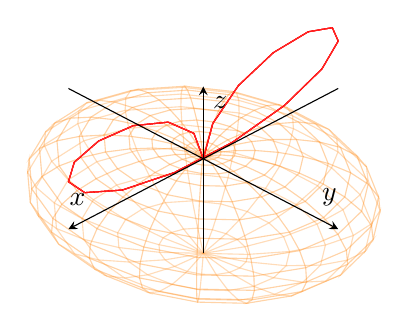
\begin{tikzpicture}
    \begin{axis}[colormap/hot2, 
        xlabel = $x$, ylabel = $y$, zlabel = $z$, 
        view = {135}{50}, 
        ticks = none, 
        axis lines=center, 
        axis on top,
        grid = major,]
    \addplot3 [surf,
        opacity = 0.2,           
        faceted color= orange,
        white,
        z buffer=sort,
        trig format plots=rad,
        samples=20, 
        domain=0:2*pi,
        y domain=0:pi,
        variable=\b,
        variable y=\a,
        grid = major,]
        ({(1- cos(a))*sin(a)*cos(b)}, {(1- cos(a))*sin(a)*sin(b)}, {(1- cos(a))*cos(a)});
    \addplot3 [surf,
        opacity = 0.2,           
        faceted color= red,
        white,
        z buffer=sort,
        trig format plots=rad,
        samples=20, 
        domain=0:pi,
        %y domain0:pi,
        variable=\a,
        %variable y=\a,
        grid = major,]
        ({2*sin(2*a)*sin(a)*cos(0)}, {2*sin(2*a)*sin(a)*sin(0)}, {2*sin(2*a)*cos(a)});
    \end{axis}
  \end{tikzpicture}

  \begin{center}
    %x^2 + y^2 + z^2 = 1
    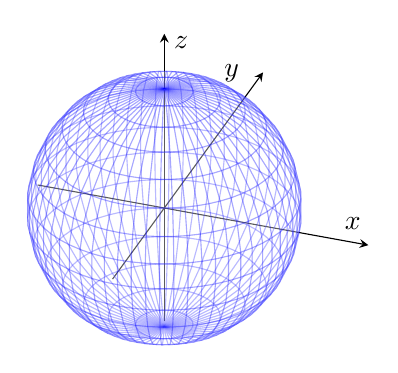
\begin{tikzpicture}
    \begin{axis}[%
        axis equal,
        width=10cm,
        height=10cm,
        axis lines = center,
        xlabel = {$x$},
        ylabel = {$y$},
        zlabel = {$z$},
        xmax=1.1,xmin=-0.5,
        ymax=1.5,ymin=-0.5,
        zmax=1.01,zmin=-0.5,
        ticks=none,
        enlargelimits=0.3,
        view/h=20,
        scale uniformly strategy=units only,
    ]
    \addplot3[%
        opacity = 0.2,
        surf,
        faceted color=blue,
    	white,
        z buffer = sort,
        samples = 31,
        variable = \u,
        variable y = \v,
        domain = 0:180,
        y domain = 0:360,
    ]
    ({cos(u)*sin(v)}, {sin(u)*sin(v)}, {cos(v)});
    \end{axis}
    \end{tikzpicture}
    \end{center}

  
\begin{comment}
    
\tableofcontents
\newpage
\chapter{HÀM NHIỀU BIẾN - ĐẠO HÀM}
\section{Hàm nhiều biến.}
\subsection{Các khái niệm cơ bản.}
\subsubsection{Hàm hai biến.}
\textbf{Định nghĩa 1.1.} Hàm hai biến là một quy luật ứng với một cặp số thực được sắp xếp thứ tự $(x, y) \in D$ ta luôn xác định được duy nhất một số thực $z=f(x, y)$.
\[
\begin{gathered}
f: D \subset \mathbb{R}^2 \rightarrow \mathbb{R} \\
(x, y) \longmapsto z=f(x, y)
\end{gathered}
\]
\begin{itemize}
    \item Tập hợp $D$ được gọi là miền xác định của hàm số $f$ và được kí hiệu $D(f)$.
    \item Tập hợp $E=\{z, \exists(x, y) \in D: z=f(x, y)\}$ được gọi là tập giá trị của hàm số $f$ và được ký hiệu $E(f)$.
\end{itemize}
%\textit{\textbf{e.g.}} Tìm miền xác định và tập giá trị của hàm số $f(x, y)=\sqrt{9-x^2-y^2}$
%\begin{enumerate}
%    \item[1.] Miền xác định của $f(x, y)$ là $D=\left\{(x, y): 9-x^2-y^2 \geqslant 0\right\}=\left\{(x, y): x^2+y^2 \leqslant 9\right\}$.
%    \item[2.] Tập giá trị của $f(x, y)$ là $E=\{z: z=\sqrt{9-x^2-y^2},(x, y) \in D\}=\{z: 0 \leqslant z \leqslant 3\}=[0,3]$ vì $z \geqslant 0$ và $\sqrt{9-x^2-y^2} \leqslant 3$
%\end{enumerate}
%\begin{center}
%    
\includegraphics[scale = 0.3]{1.png}
%\end{center}
\subsubsection{Đồ thị hàm hai biến.}
\textbf{Định nghĩa 1.2.} Đồ thị của hàm hai biến $z=f(x, y)$ là tập hợp tất cả những điểm $(x, y, z) \in \mathbb{R}^3$ sao cho $z=f(x, y)$ và $(x, y) \in D$.

%Đồ thị của hàm một biến $y=f(x)$ là một đường cong, còn đồ thị của hàm hai biến $z=f(x, y)$ là một mặt cong.
%\begin{center}
%    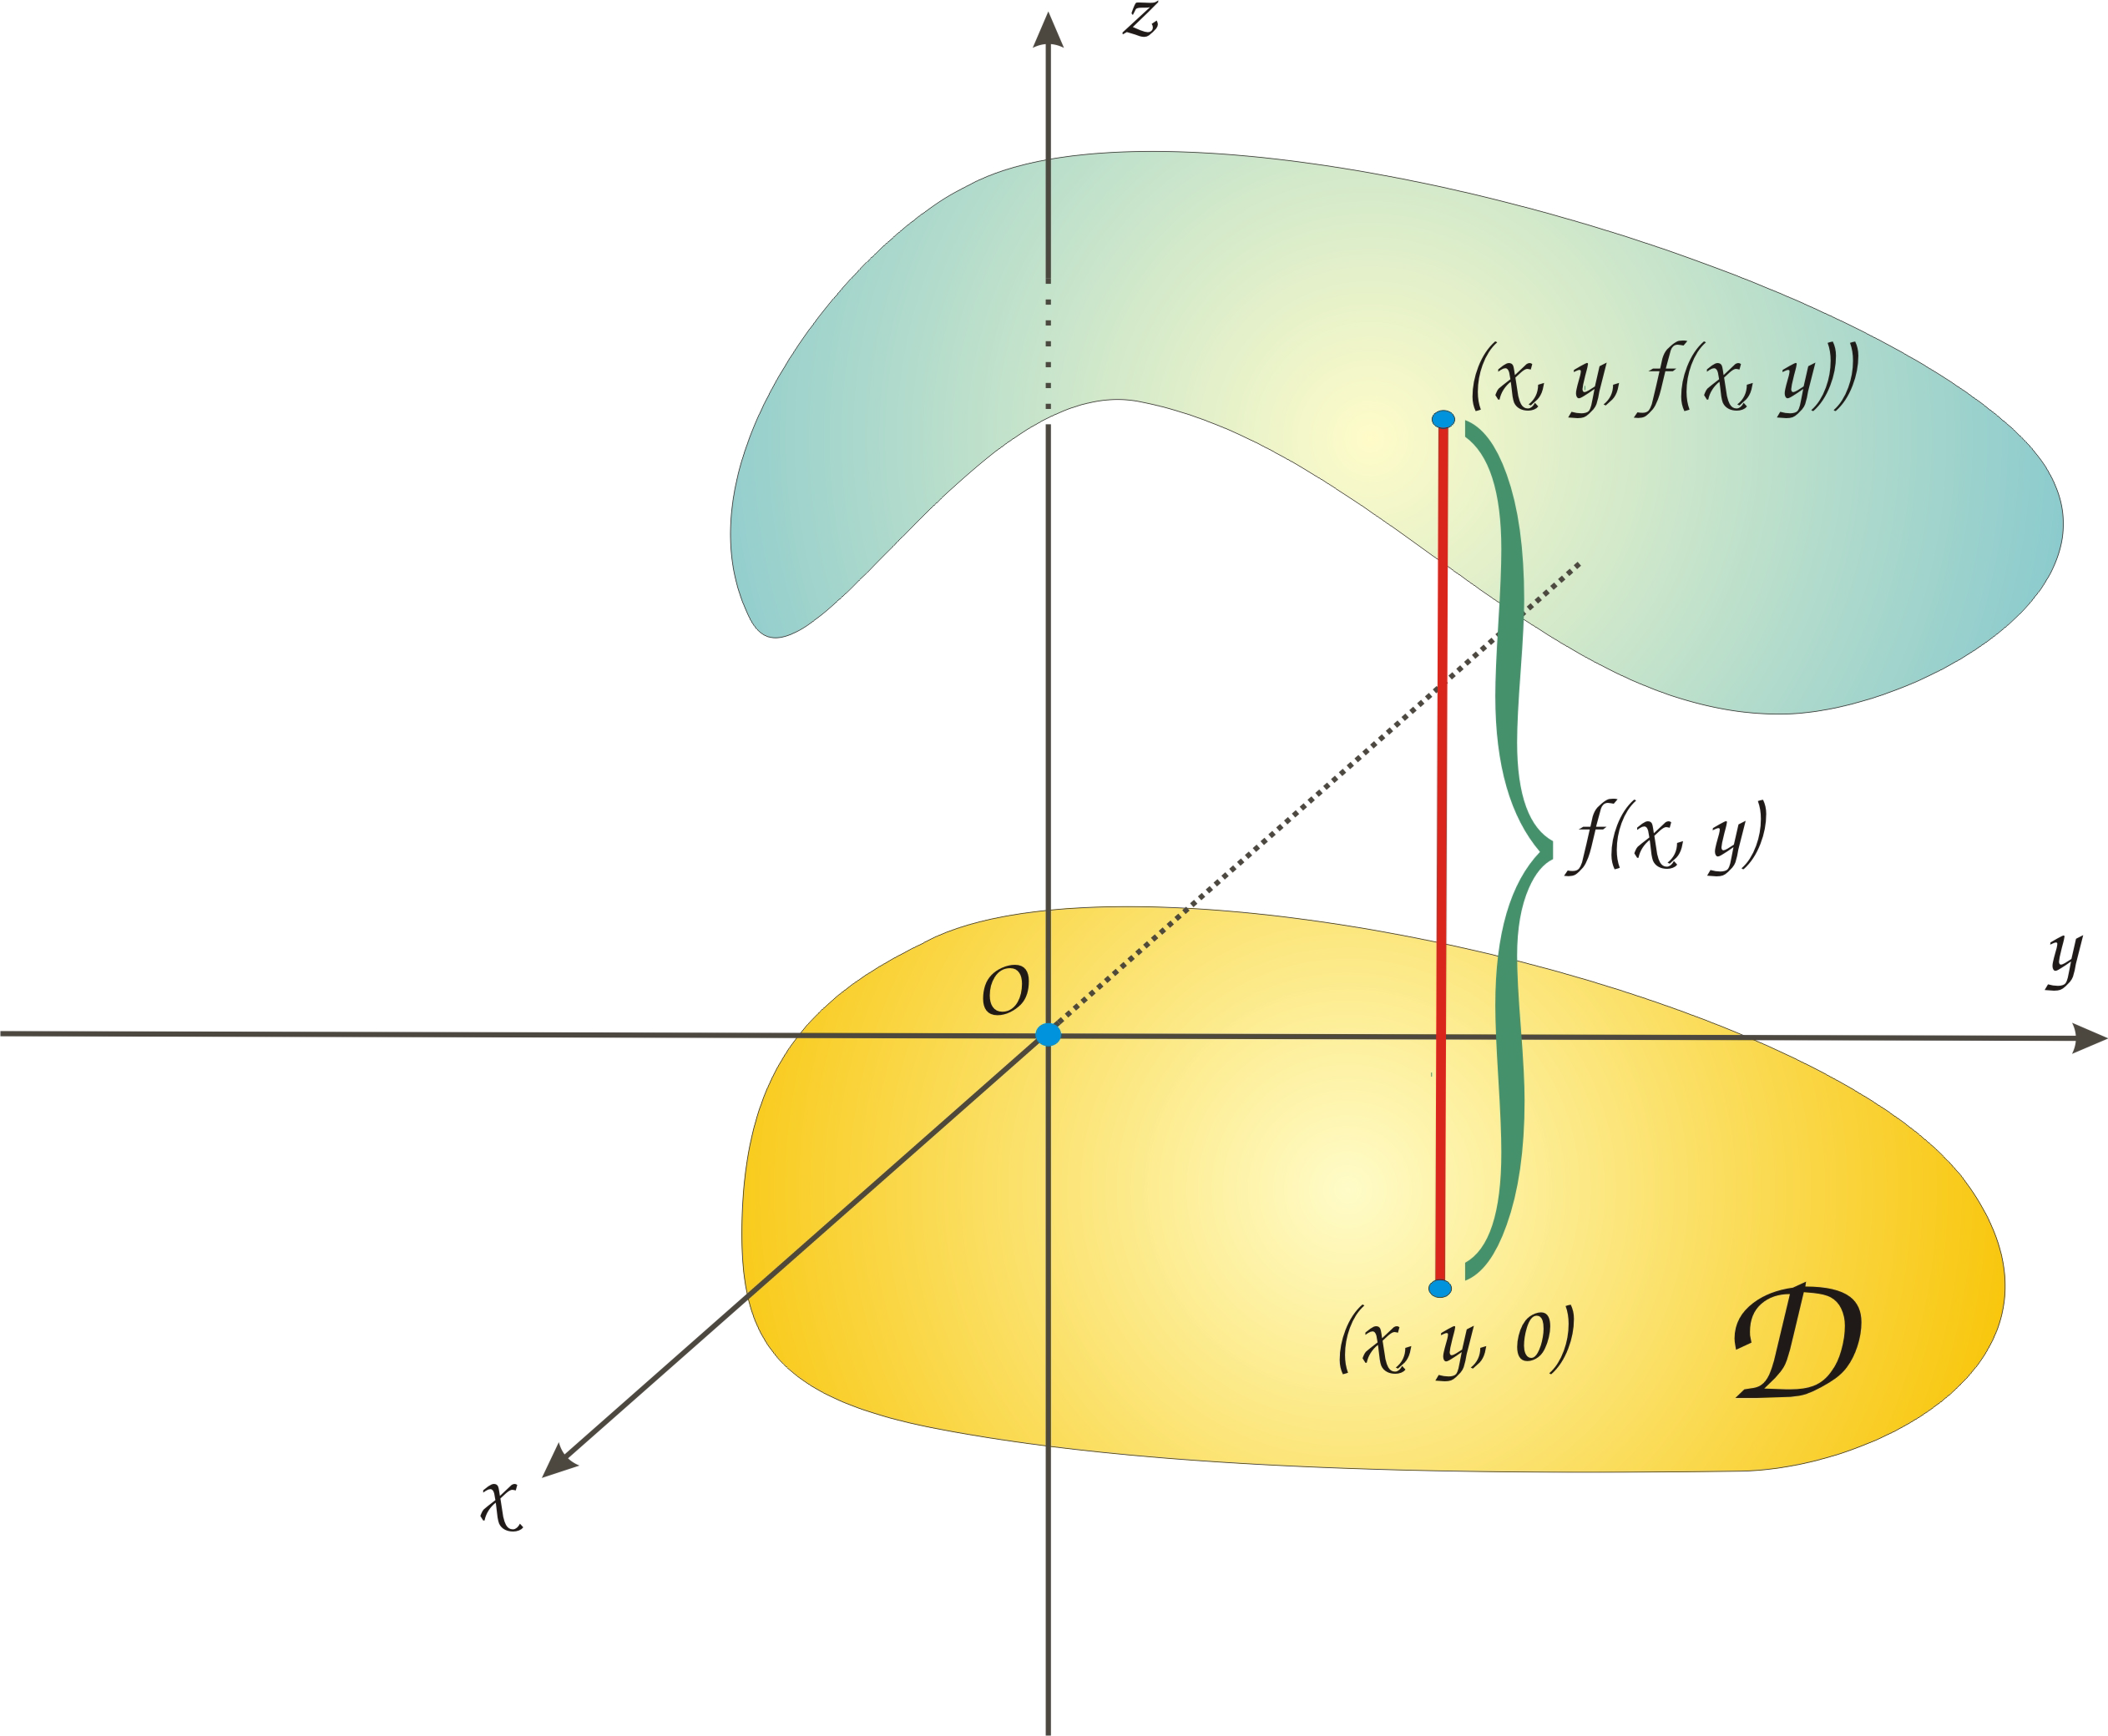
\includegraphics[scale = 0.15]{2.png}
%\end{center}
\subsection{Đường mức.}
\textbf{Định nghĩa 1.3.} Đường mức của hàm số $z=f(x, y)$ là đường cong có phương trình là $f(x, y)=k$, với $k$ là hằng số (thuộc tập giá trị của $f(x, y)$).
\begin{center}
    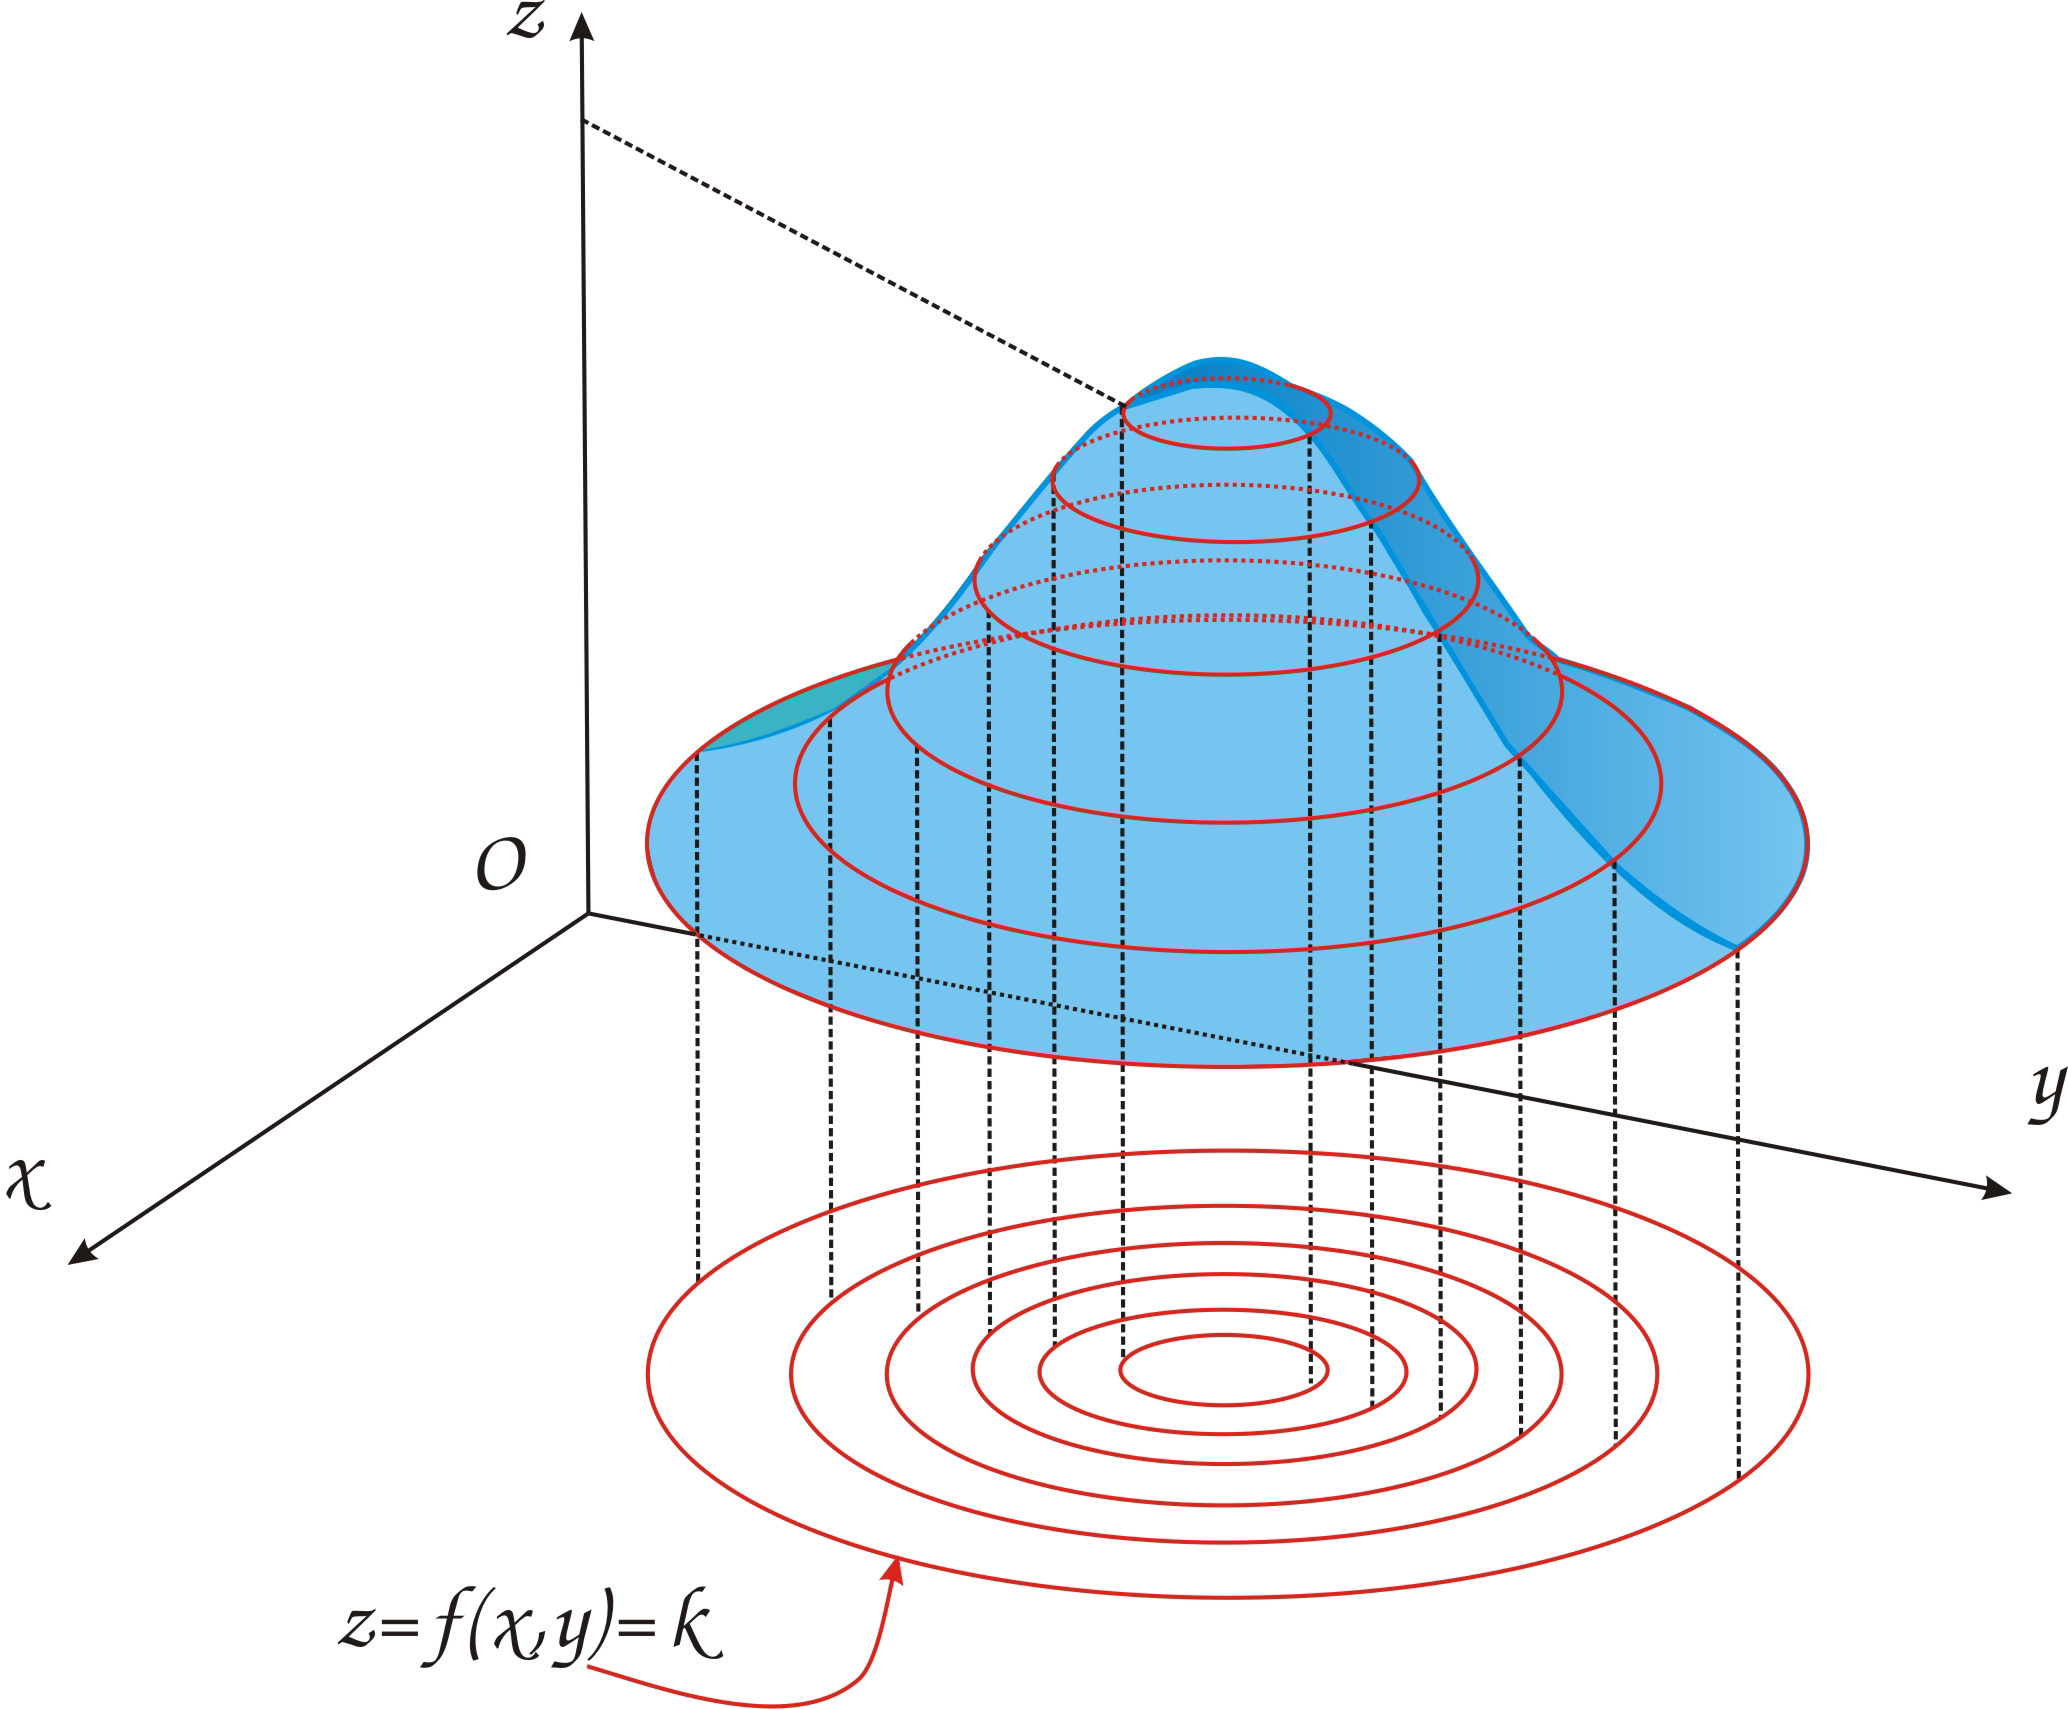
\includegraphics[scale = 0.18]{3.png}
\end{center}
%Chú ý. Từ định nghĩa của hàm nhiều biến thì các đường đẳng trị sẽ không cắt nhau vì ứng với mỗi điểm $(x, y)$ ta luôn xác định được duy nhất một giá trị của hàm số $z=f(x, y)$. Thật vậy, giả sử nếu hai đường đẳng trị $z=k_1$ và $z=k_2\left(k_1 \neq k_2\right)$ khác nhau cắt nhạ thì ứng với một điểm $(x, y)$ có hai giá trị khác nhau $z=k_1$ và $z_0=k_2$.
\subsection{Hàm nhiều biến.}
\textbf{Định nghĩa 1.4.} Hàm $n$ biến là một quy tắc $f$ sao cho ứng với mỗi bộ số thực có thứ tự $(x_1, x_2, \ldots, x_n) \in D \subset \mathbb{R}^n$ luôn có duy nhất một số thực $z=f(x_1, x_2, \ldots, x_n)$.
\[
\begin{gathered}
f: D \subset \mathbb{R}^n \rightarrow \mathbb{R} \\
\left(x_1, x_2, \ldots, x_n\right) \longmapsto f\left(x_1, x_2, \ldots, x_n\right)
\end{gathered}
\]
%hoặc $u=f(x)=f\left(x_1, x_2, \ldots, x_n\right)$. Tập hợp $D$ được gọi là miền xác định của hàm số này và được kí hiệu $D(f)$.
\begin{comment}
\subsection{Đường thẳng và mặt phẳng trong không gian.}
\subsubsection{Đường thẳng.}
Cho $(d)$ là đường thẳng đi qua $M_0\left(x_0, y_0, z_0\right)$ và song song với véc tơ $\vec{a}=\left(a_1, a_2, a_3\right)$. Vậy $(d)$ là tập hợp tất cả những điểm $M(x, y, z)$ sao cho $\overrightarrow{M_0 M} \uparrow \uparrow \vec{a}$.

Do đó nếu $M \in(d)$ thì
\[
\frac{x-x_0}{a_1}=\frac{y-y_0}{a_2}=\frac{z-z_0}{a_3}=t,(t \in \mathbb{R}) .
\]
Từ đó, ta được phương trình tham số của đường thẳng (d).
\[
\begin{cases}
    x = x_0 + a_1 t\\
    y = y_0 + a_2 t\\
    z = z_0 + a_3 t\\
\end{cases}
\]
\subsubsection{Mặt phẳng.}
Cho $(P)$ là mặt phẳng đi qua điểm $M_0\left(x_0, y_0, z_0\right)$ và vuông góc với véc tơ $\vec{n}=\left(n_1, n_2, n_3\right)$. Khi đó $(P)$ là tập hợp những điểm $M(x, y, z)$ sao cho $\overrightarrow{M_0 M} \perp \vec{n}$. Do đó phương trình của mặt phẳng $(P)$ là
\[
n_1\left(x-x_0\right)+n_2\left(y-y_0\right)+n_3\left(z-z_0\right)=0 .
\]
\subsection{Các mặt bậc hai.}
\subsubsection{Mặt Ellipsoid.}
Phương trình chính tắc của mặt Ellipsoid
\[
    \frac{x^2}{a^2}+\frac{y^2}{b^2}+\frac{z^2}{c^2}=1, \quad(a, b, c \in \mathbb{R})
\]
\begin{itemize}
    \item Mọi mặt phẳng $z=k$ cắt mặt Ellipsoid theo đường Ellipse $\dfrac{x^2}{a^2}+\dfrac{y^2}{b^2}=1-\dfrac{k^2}{c^2}$, với điều kiện $-c<k<c$.
    \item Mọi mặt phẳng $y=k$ cắt mặt Ellipsoid theo đường Ellipse $\dfrac{x^2}{a^2}+\dfrac{z^2}{c^2}=1-\dfrac{k^2}{b^2}$, với điều kiện $-b<k<b$.
    \item Mọi mặt phẳng $x=k$ cắt mặt Ellipsoid theo đường Ellipse $\dfrac{y^2}{b^2}+\dfrac{z^2}{c^2}=1-\dfrac{k^2}{a^2}$, với điều kiện $-a<k<a$.
\end{itemize}
\begin{center}
    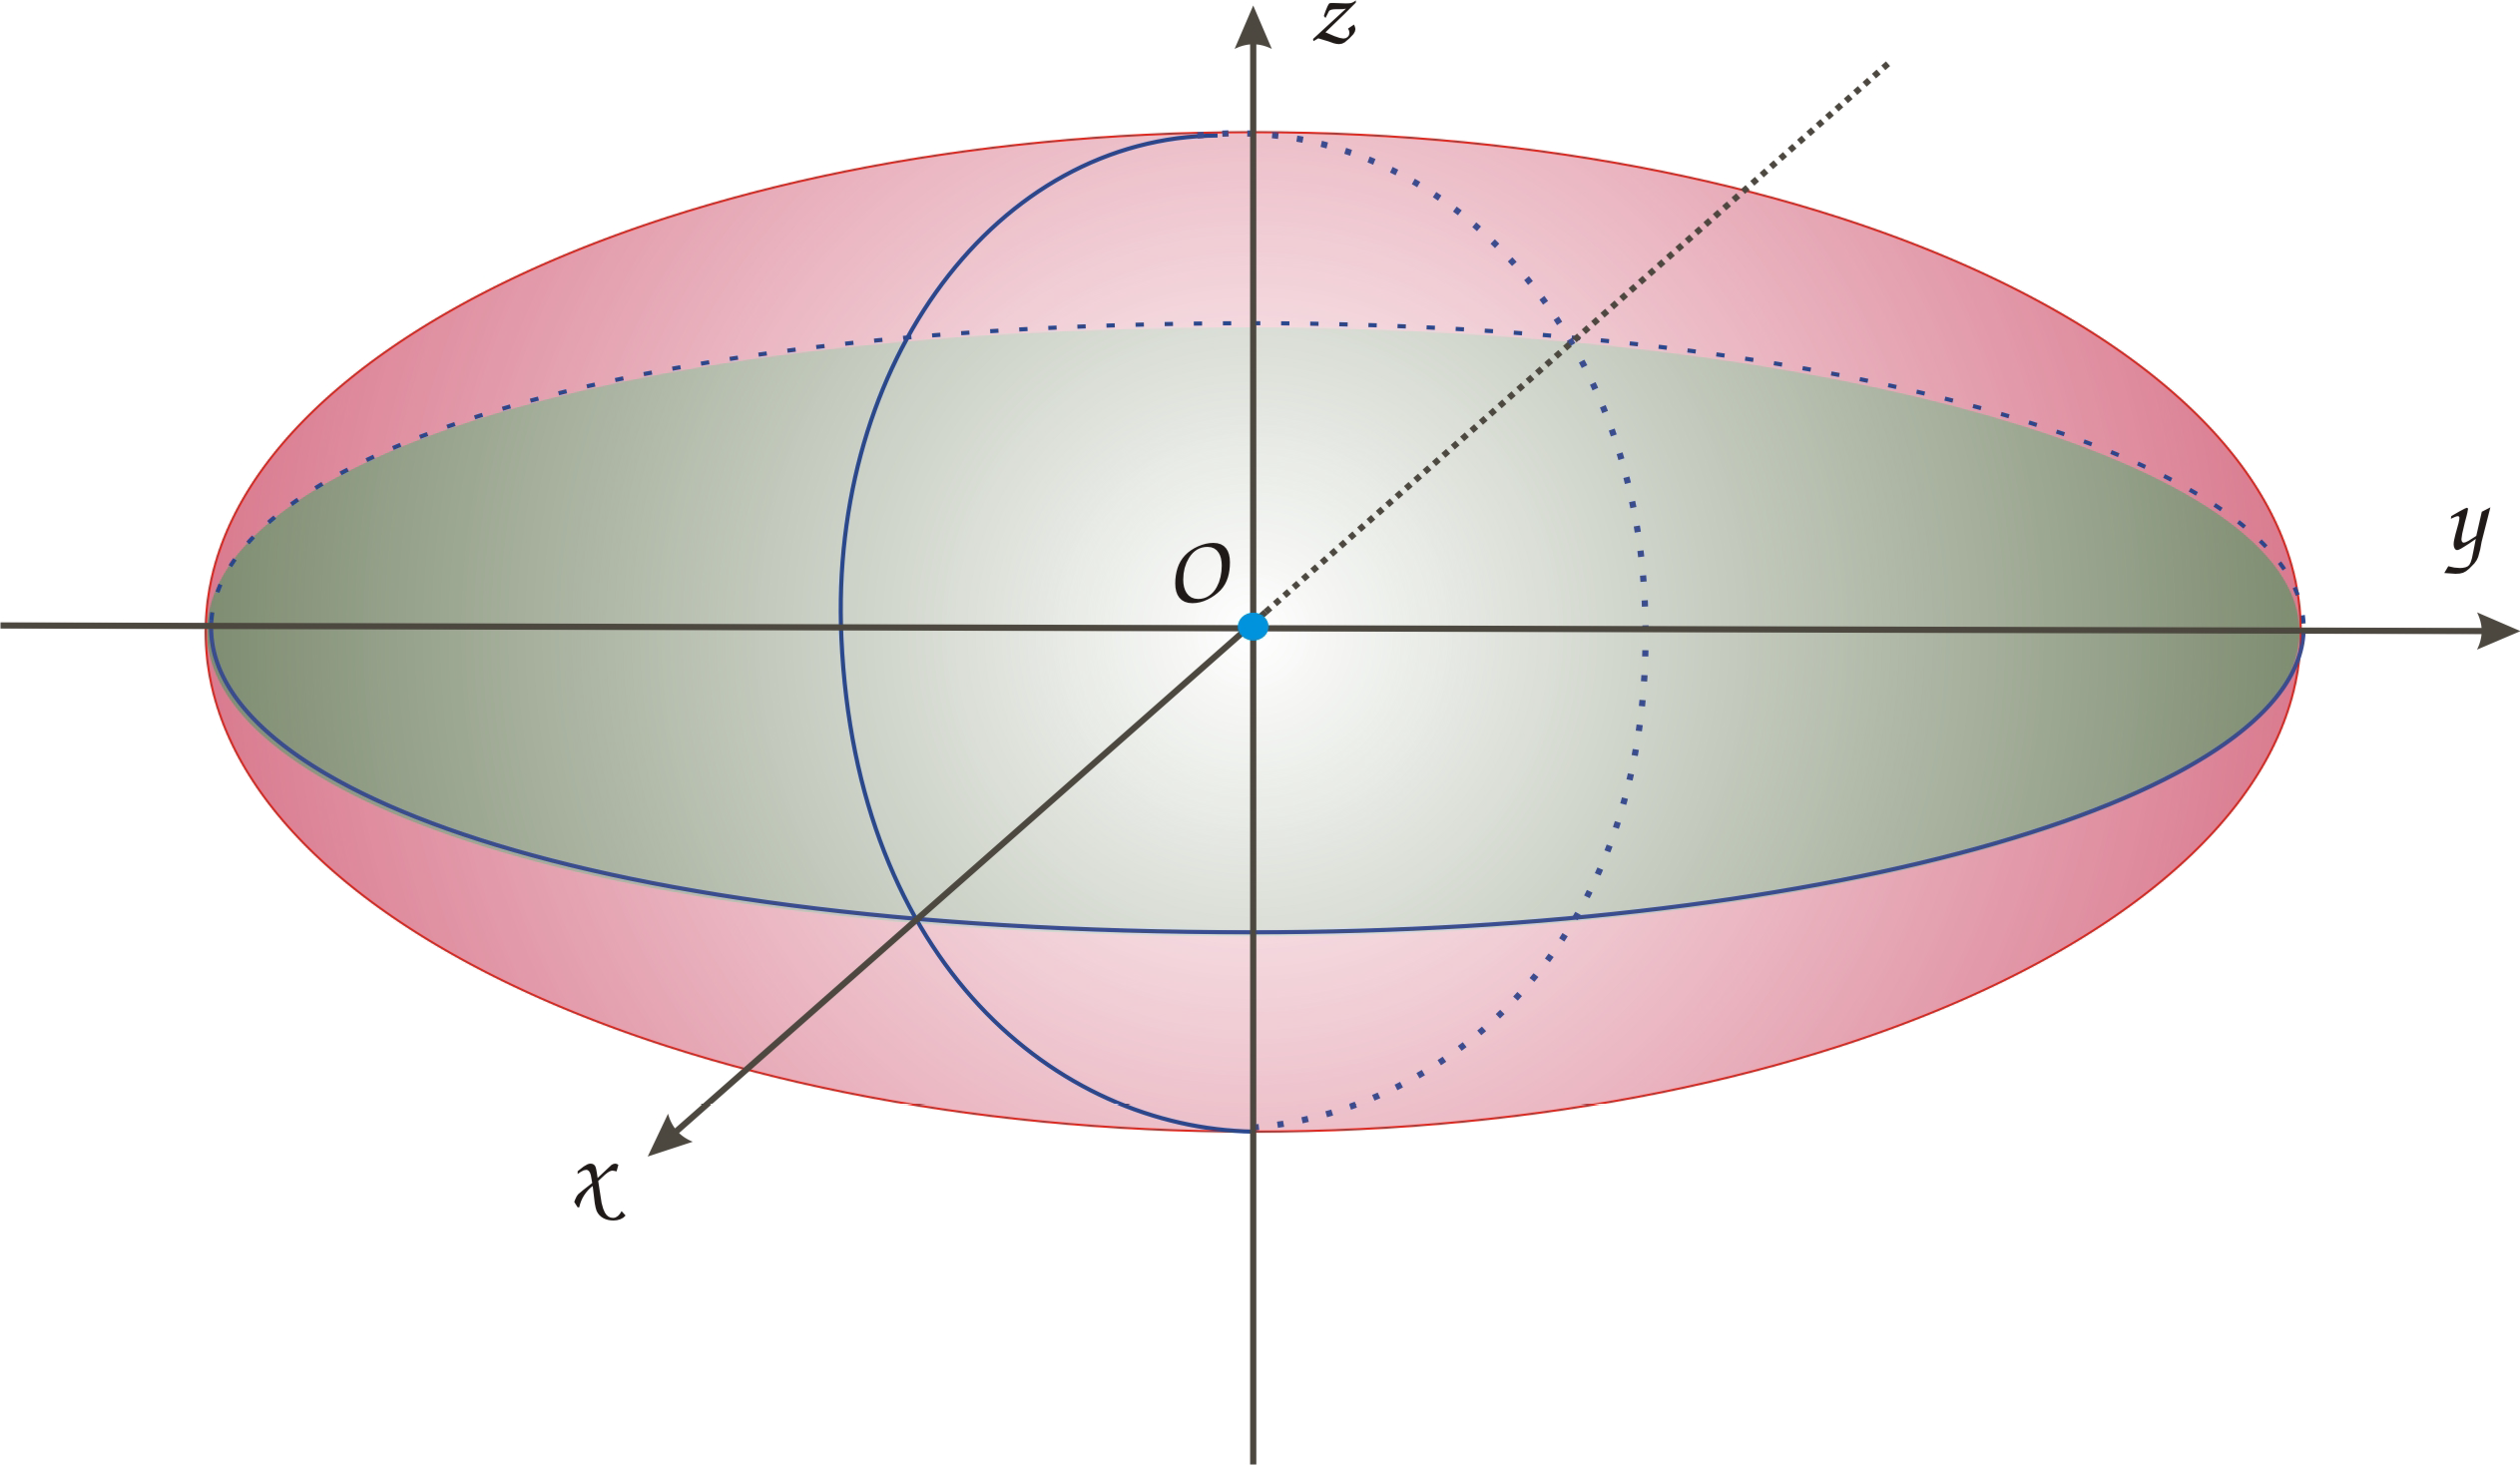
\includegraphics[scale = 0.25]{4.png}
    \captionof*{figure}{Đồ thị mặt Ellipsoid}
\end{center}
Như vậy, mọi mặt cắt đều là Ellipse nên mặt cong này được gọi là mặt Ellipsoid. Khi $a=b=c=R$ thì mặt Ellipsoid sẽ trở thành mặt cầu tâm $(0,0,0)$ bán kính $R$.
\subsubsection{Mặt Paraboloid Elliptic.}
Phương trình chính tắc mặt Paraboloid Elliptic
\[
    z = \frac{x^2}{a^2} + \frac{y^2}{b^2}    
\]
\begin{itemize}
    \item Mọi mặt phẳng $z=k$ cắt mặt Paraboloid Elliptic theo đường Ellipse $\dfrac{x^2}{a^2}+\dfrac{y^2}{b^2}=k$, với điều kiện $k>0$.
    \item Mọi mặt phẳng $y=k$ cắt mặt Paraboloid Elliptic theo đường Parabol $z = \dfrac{x^2}{a^2} + \dfrac{k^2}{b^2}$.
    \item Mọi mặt phẳng $x=k$ cắt mặt Paraboloid Elliptic theo đường Parabol $z = \dfrac{k^2}{a^2} + \dfrac{y^2}{b^2}$.
\end{itemize}
\begin{center}
    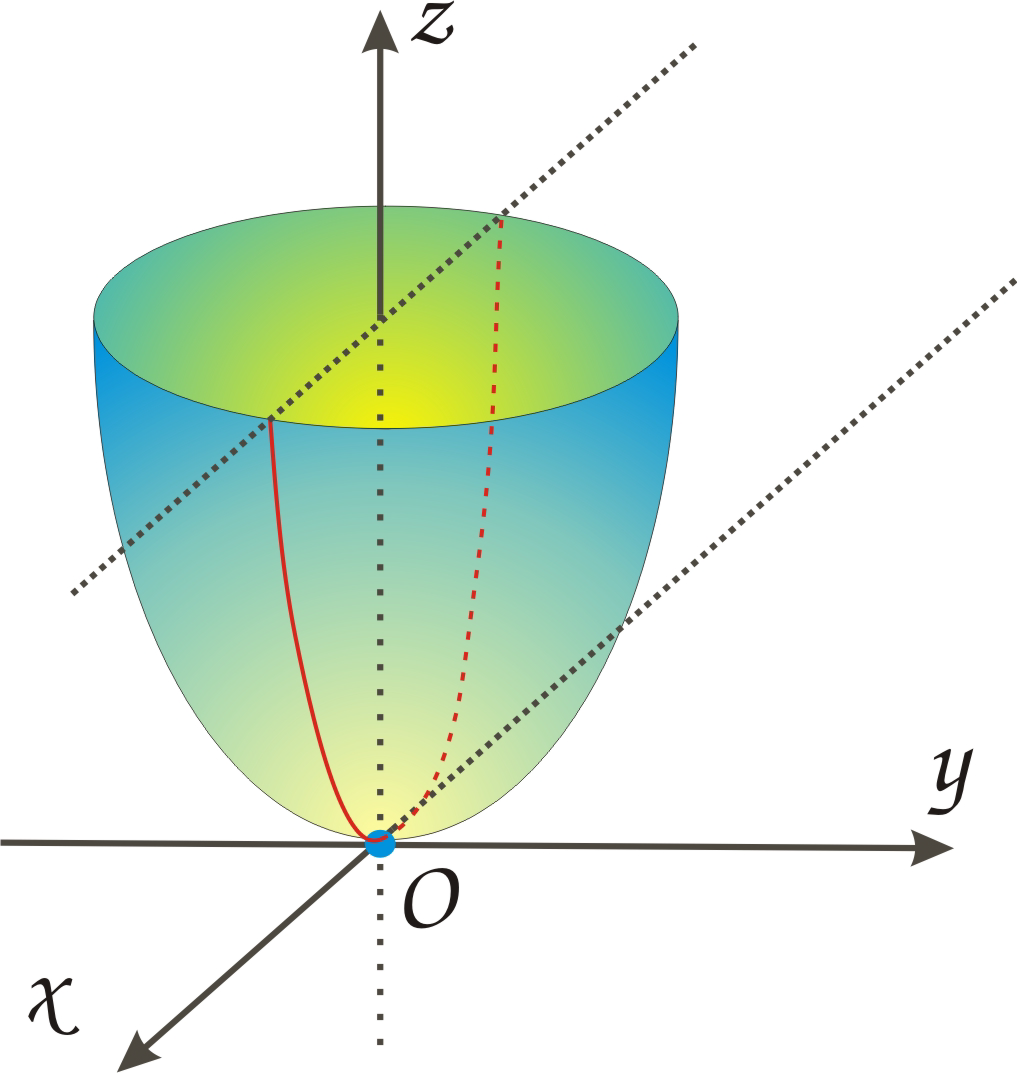
\includegraphics[scale = 0.25]{5.png}
    \captionof*{figure}{Đồ thị mặt Paraboloid Elliptic}
\end{center}
Như vậy, mặt cắt là những Parabol và Ellipse nên mặt cong này được gọi là mặt Paraboloid Elliptic.
\subsubsection{Mặt Paraboloid Hyperbolic.}
Phương trình chính tắc của mặt Paraboloid Hyperbolic
\[
    z =   \frac{x^2}{a^2} - \frac{y^2}{b^2}      
\]
\begin{itemize}
    \item Mọi mặt phẳng $z=k$ cắt mặt Paraboloid Hyperbolic theo đường Hyperbol $\dfrac{x^2}{a^2} - \dfrac{y^2}{b^2}=k$.
    \item Mọi mặt phẳng $y=k$ cắt mặt Paraboloid Hyperbolic theo đường Parabol $z = \dfrac{x^2}{a^2} - \dfrac{k^2}{b^2}$.
    \item Mọi mặt phẳng $x=k$ cắt mặt Paraboloid Hyperbolic theo đường Parabol $z = \dfrac{k^2}{a^2} - \dfrac{y^2}{b^2}$.
\end{itemize}
\begin{center}
    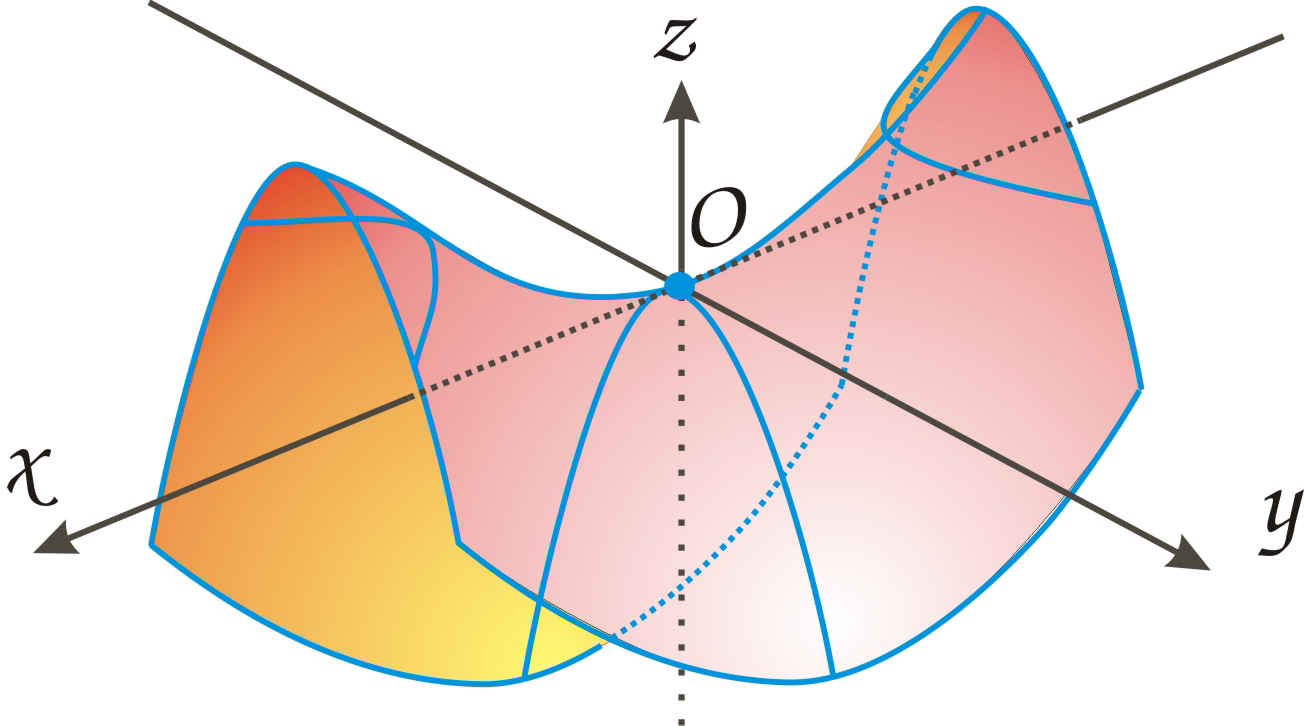
\includegraphics[scale = 0.25]{6.png}
    \captionof*{figure}{Đồ thị mặt Paraboloid Hyperbolic}
\end{center}
Như vậy, mặt cắt là những Parabol và Hyperbol nên mặt cong này được gọi là mặt Paraboloid Hyperbolic hay còn được gọi là hình yên ngựa.
\subsubsection{Mặt Hyperboloid.}
\textbf{Phương trình chính tắc của mặt Hyperboloid một tầng}
\[
    \frac{x^2}{a^2}+\frac{y^2}{b^2}-\frac{z^2}{c^2}=1
\]
\begin{itemize}
    \item Mọi mặt phẳng $z=k$ cắt mặt Hyperboloid một tầng theo đường Ellipse $\dfrac{x^2}{a^2}+\dfrac{y^2}{b^2}=1 + \dfrac{k^2}{c^2}$.
    \item Mọi mặt phẳng $y=k$ cắt mặt Hyperboloid một tầng theo đường Hyperbol $\dfrac{x^2}{a^2} - \dfrac{z^2}{c^2} = 1 - \dfrac{k^2}{b^2}$.
    \item Mọi mặt phẳng $x=k$ cắt mặt Hyperboloid một tầng theo đường Hyperbol $\dfrac{y^2}{b^2} - \dfrac{z^2}{c^2} = 1 - \dfrac{k^2}{a^2}$.
\end{itemize}
\begin{center}
    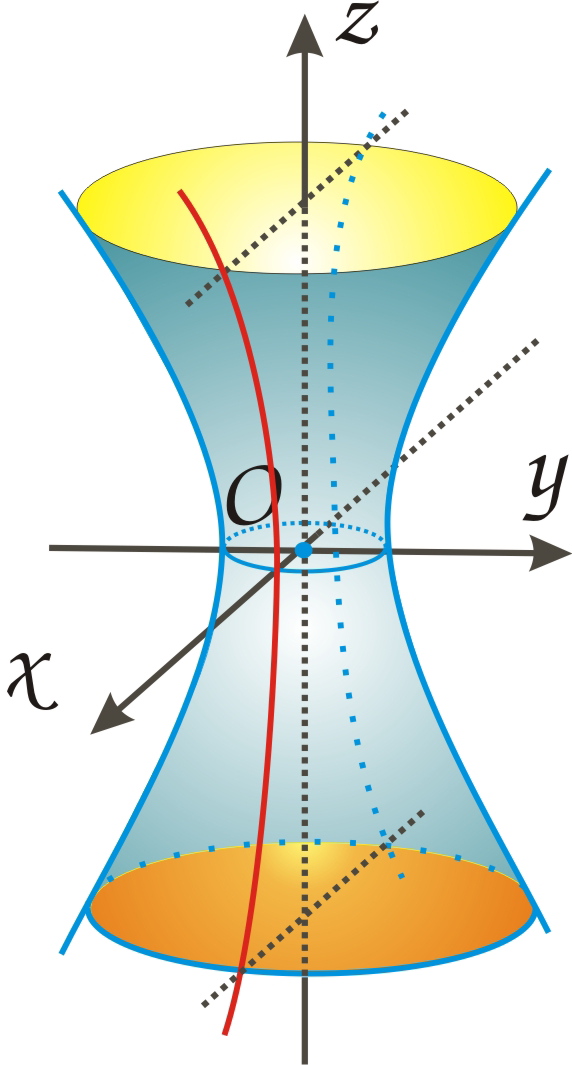
\includegraphics[scale = 0.3]{7.png}
    \captionof*{figure}{Đồ thị mặt Hyperboloid một tầng}
\end{center}
Như vậy, mặt cắt là những Hyperbol và Ellipse nên mặt cong này được gọi là Hyperboloid một tầng.

\textbf{Phương trình chính tắc của mặt Hyperboloid hai tầng}
\[
    \frac{x^2}{a^2}+\frac{y^2}{b^2}-\frac{z^2}{c^2}=-1
\]
\begin{itemize}
    \item Mọi mặt phẳng $z=k$ cắt mặt Hyperboloid hai tầng theo đường Ellipse
        \[\dfrac{x^2}{a^2}+\dfrac{y^2}{b^2}= -1 + \dfrac{k^2}{c^2}\]
    với điều kiện $k>c$ hoặc $k<-c$.
    \item Mọi mặt phẳng $y=k$ cắt mặt Hyperboloid hai tầng theo đường Hyperbol
        \[\dfrac{x^2}{a^2} - \dfrac{z^2}{c^2} = -1 - \dfrac{k^2}{b^2}\]
    \item Mọi mặt phẳng $x=k$ cắt mặt Hyperboloid hai tầng theo đường Hyperbol 
        \[\dfrac{y^2}{b^2} - \dfrac{z^2}{c^2} = -1 - \dfrac{k^2}{a^2}\]
\end{itemize}
\begin{center}
    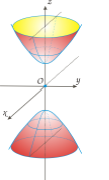
\includegraphics[scale = 1.5]{8.png}
    \captionof*{figure}{Đồ thị mặt Hyperboloid hai tầng}
\end{center}
Như vậy, mặt cắt là những Hyperbol và Ellipse nên mặt cong này được gọi là Hyperboloid hai tầng. Trong trường hợp $k>c$ hoặc $k<-c$ ta được mặt Hyperboloid một phía.
\subsubsection{Mặt trụ.}
\begin{enumerate}
    \item[1.] Phương trình chính tắc của mặt trụ Ellipse
        \[\frac{x^2}{a^2} + \frac{y^2}{b^2} = 1, z \in \mathbb{R}\]
    Trong phương trình mặt trụ này không có biến $z$. Điều này có nghĩa là mọi mặt phẳng $z = k$ (song song với mặt phẳng xOy) sẽ cắt mặt trụ Ellipse theo đường Ellipse $\dfrac{x^2}{a^2} + \dfrac{y^2}{b^2} = 1$. Mặt trụ này được gọi là mặt trụ Ellipse vì nó được tạo bới rất nhiều đường Ellipse giống nhau.
    \begin{center}
        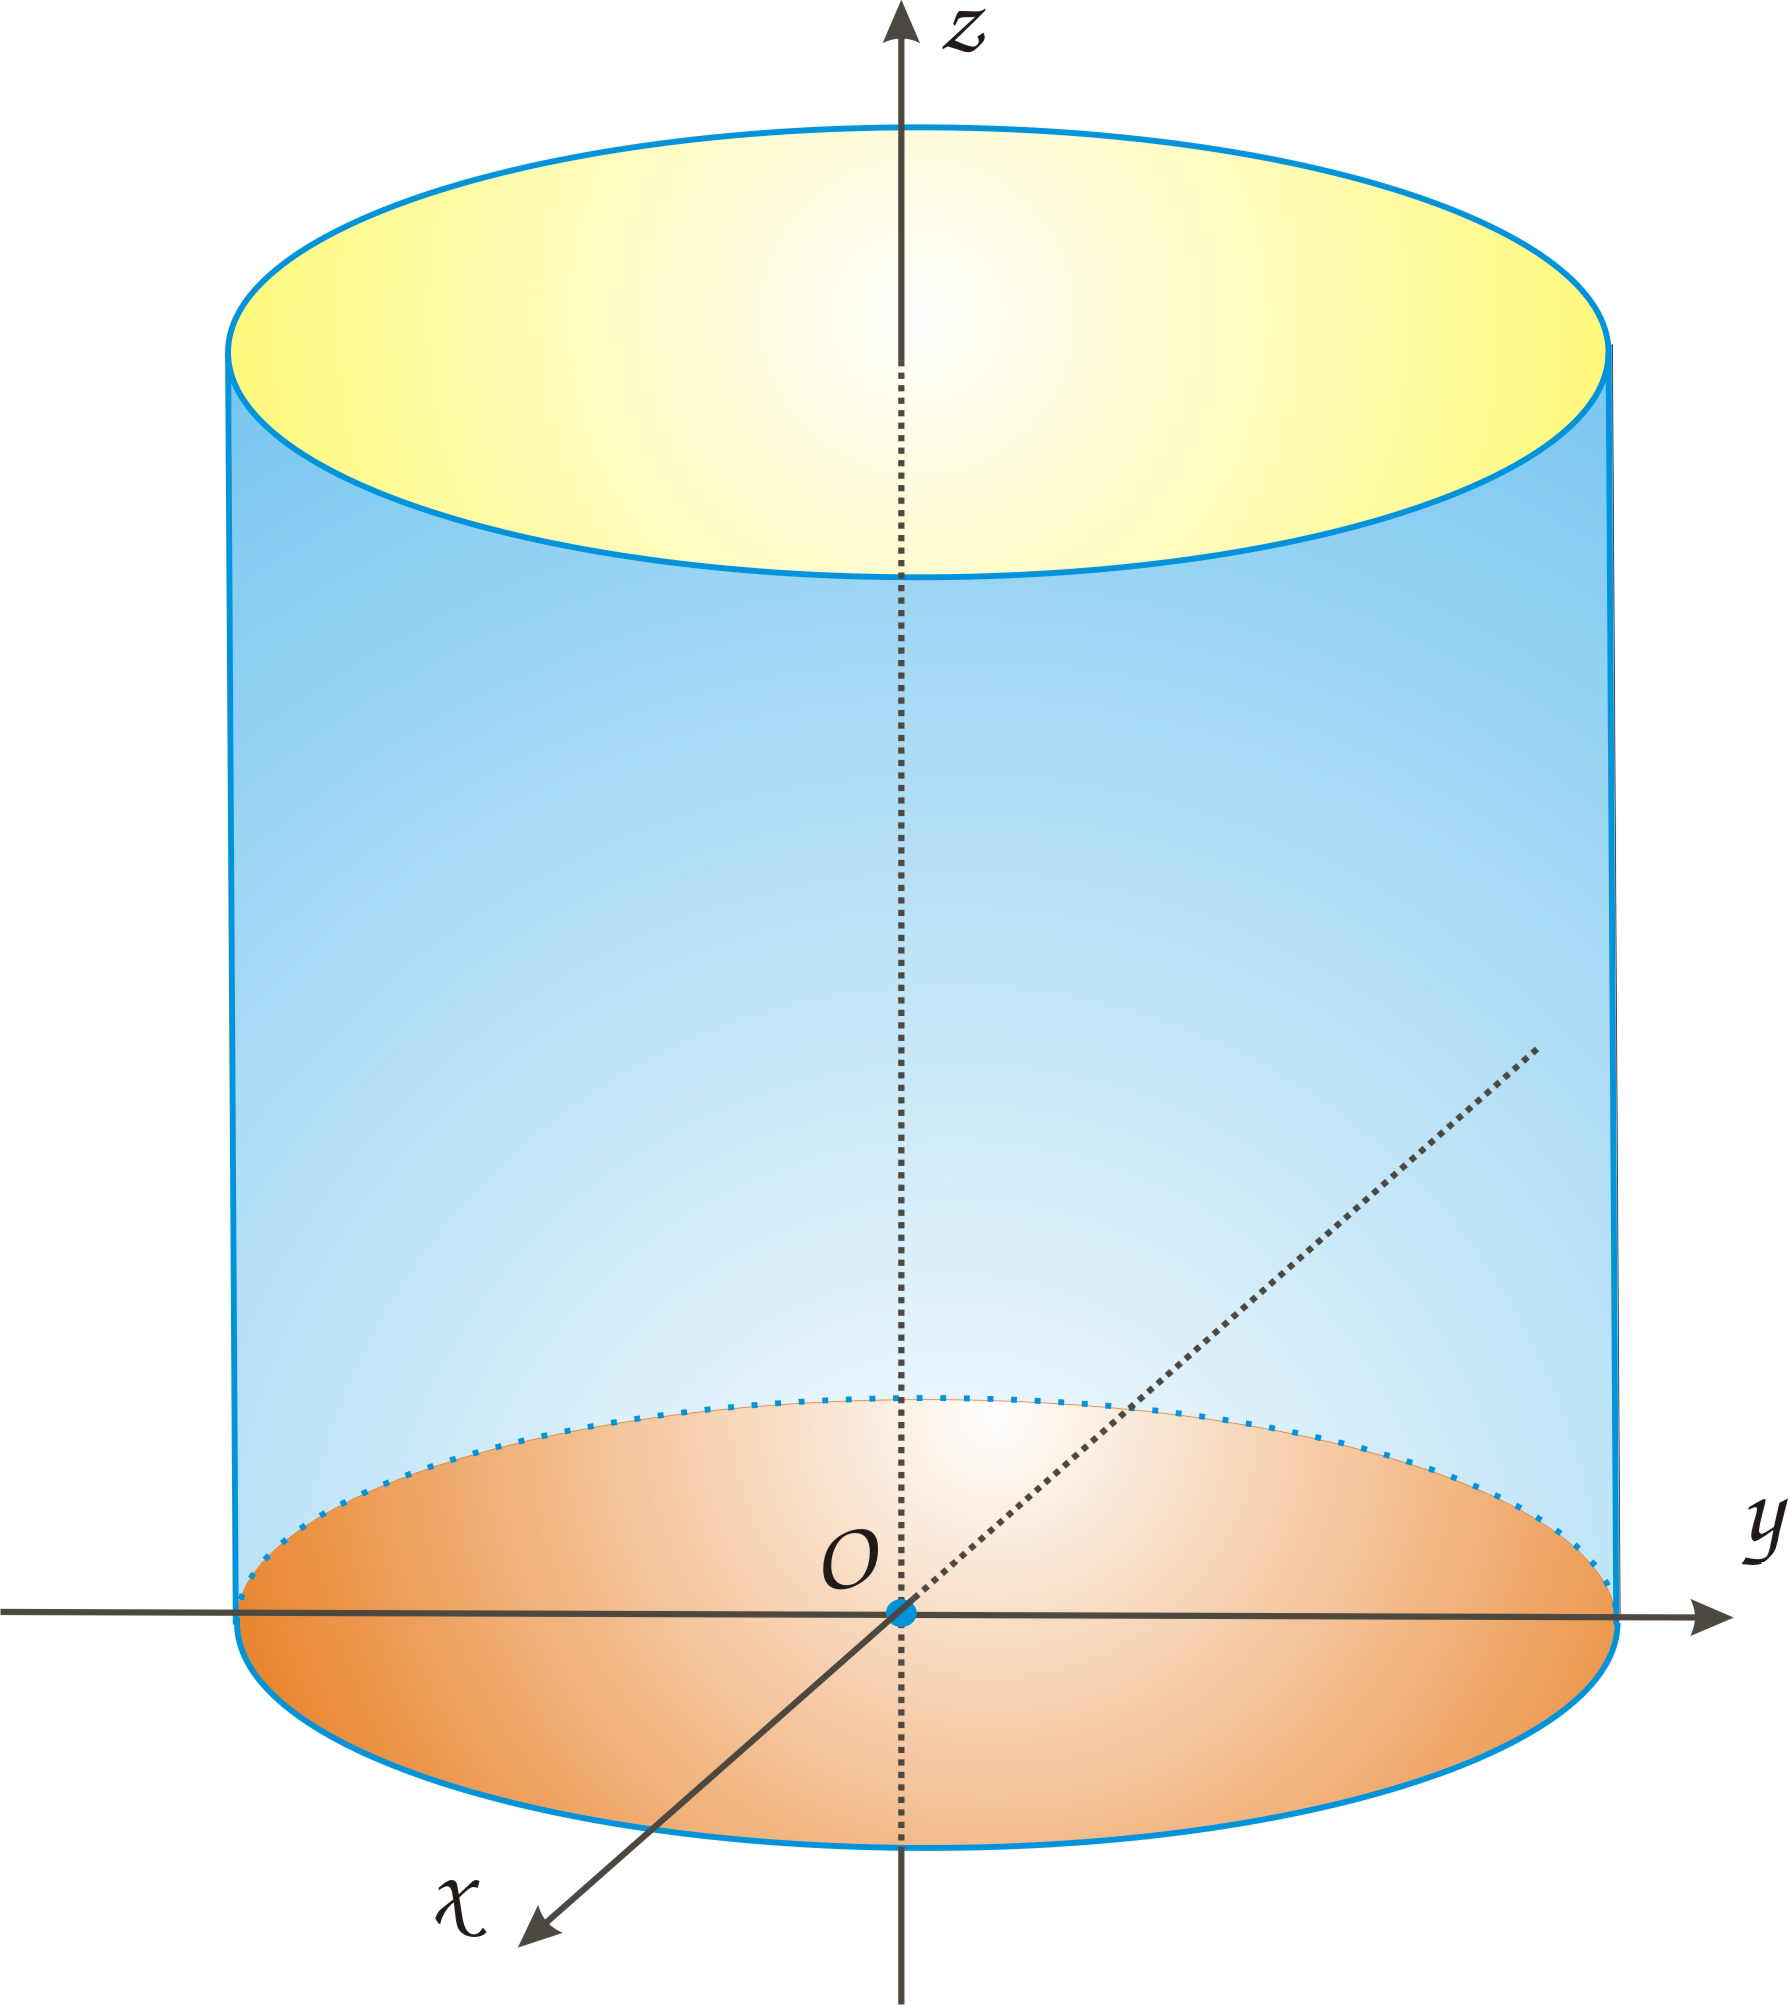
\includegraphics[scale = 0.2]{9.png}
        \captionof*{figure}{Đồ thị mặt trụ Ellipse}
    \end{center}
    \item[2.] Khi $a=b=R$ ta có phương trình chính tắc của mặt trụ tròn
        \[x^2 + y^2 = R^2,z \in \mathbb{R}\]
    \item[3.] Phương trình chính tắc của mặt trụ Parabol
        \[y^2 = 2px, z \in \mathbb{R}\]
        \begin{center}
            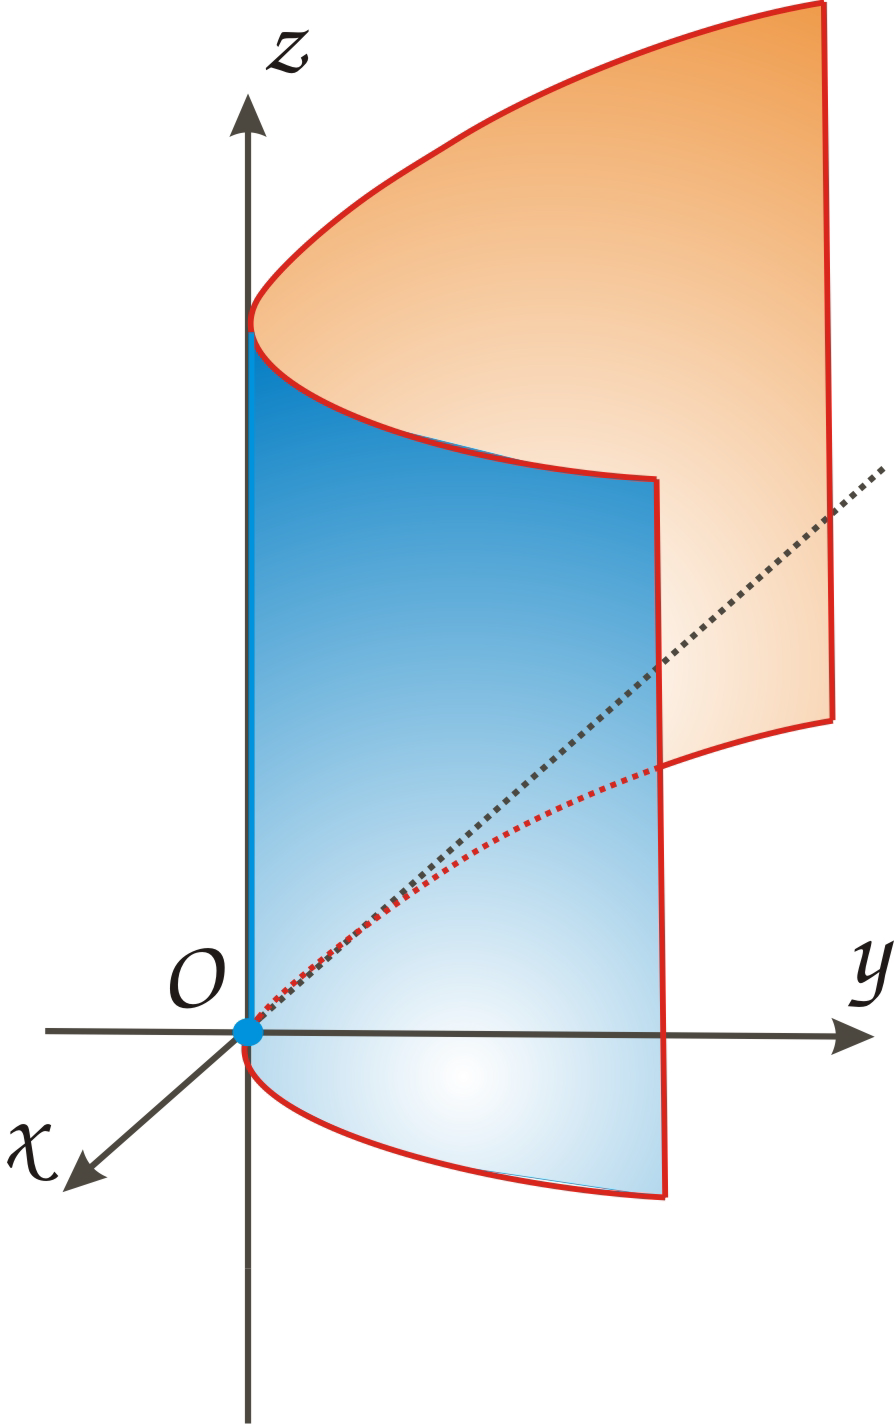
\includegraphics[scale = 0.3]{10.png}
            \captionof*{figure}{Đồ thị mặt trụ Parabol}
        \end{center}
        Trong phương trình mặt trụ Parabol không có biến $z$. Điều này có nghĩa là mọi mặt phẳng $z = k$ (song song với mặt phẳng xOy) sẽ cắt mặt trụ Parabol theo đường Parabol $y^2 = 2px$. Mặt trụ này được gọi là mặt trụ Parabol vì nó được tạo bởi rất nhiều đường Parabol giống nhau.
\end{enumerate}
\subsubsection{Mặt nón hai phía.}
Phương trình chính tắc của mặt nón hai phía
\[
    \frac{x^2}{a^2}+\frac{y^2}{b^2}=\frac{z^2}{c^2}
\]
\begin{center}
    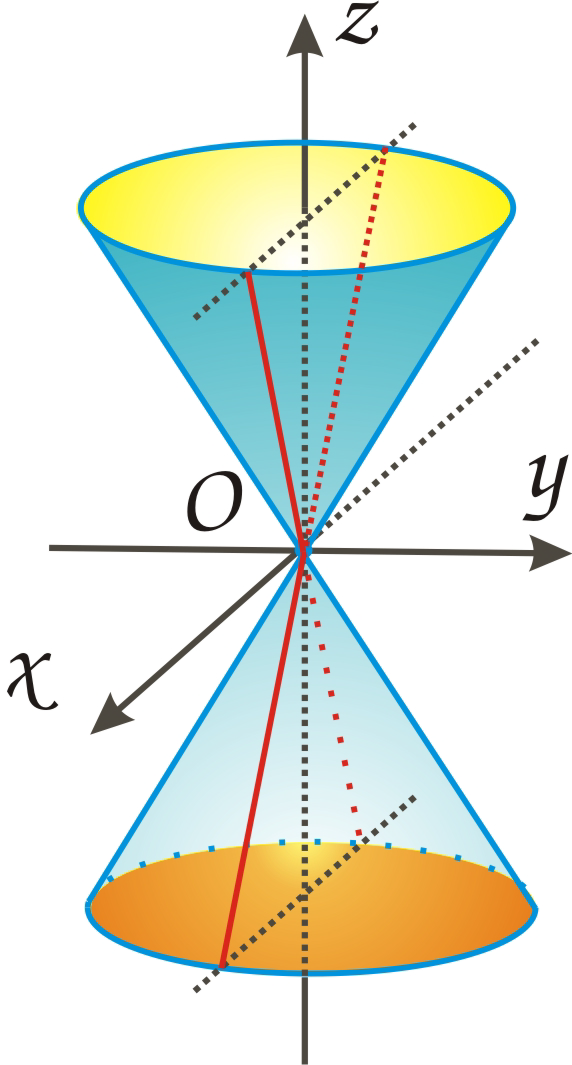
\includegraphics[scale = 0.35]{11.png}
    \captionof*{figure}{Đồ thị mặt Hyperboloid hai tầng}
\end{center}
\begin{itemize}
    \item Mọi mặt phẳng $z=k$ cắt mặt nón hai phía theo đường Ellipse $\dfrac{x^2}{a^2}+\dfrac{y^2}{b^2}=\dfrac{k^2}{c^2}$.
    \item Mọi mặt phẳng $y=k$ cắt mặt nón hai phía theo đường Hyperbol $\dfrac{x^2}{a^2} - \dfrac{z^2}{c^2} = - \dfrac{k^2}{b^2}$, với $k \neq 0$; cắt mặt nón hai phía theo đường thẳng $\dfrac{z}{c} = \pm \dfrac{x}{a},$ với $k=0$.
    \item Mọi mặt phẳng $y=k$ cắt mặt nón hai phía theo đường Hyperbol $\dfrac{y^2}{b^2} - \dfrac{z^2}{c^2} = - \dfrac{k^2}{a^2}$, với $k \neq 0$; cắt mặt nón hai phía theo đường thẳng $\dfrac{z}{c} = \pm \dfrac{y}{b},$ với $k=0$.
\end{itemize}
Như vậy, mặt cắt là những Hyperbol, Ellipse và đường thẳng, tạo nên hình nón nên mặt cong này được gọi là mặt nón hai phía. Trong trường hợp nếu $z > 0$ hoặc $z < 0$ thì ta được mặt nón một phía.    
\section{Đạo hàm riêng và vi phân.}
\begin{comment}
\subsection{Giới hạn và tính liên tục của hàm nhiều biến.}
\textbf{Định nghĩa 2.1.} Số $L \in \mathbb{R}$ được gọi là giới hạn của hàm số $f(x,y)$ khi $(x,y)$ tiến đến $(a,b) \in D,$
\[
    \lim_{(x,y) \to (a,b)} f(x,y) = L,    
\]
nếu như $\forall x > 0$ tồn tại $\delta > 0$ sao cho với mọi $(x,y) \in D : 0 < \sqrt{(x-a)^2 + (y-b)^2} < \delta$ luôn có $|f(x,y) - L|< \varepsilon$.

\DN \textbf{2.2.} Số $L \in \mathbb{R}$ được gọi là giới hạn của hàm số $f(x,y)$ khi $(x,y)$ tiến đến $(a,b) \in D,$
\[
    \lim_{(x,y) \to (a,b)} f(x,y) = L,    
\]
nếu như $\forall \{(x_n),(y_n)\} \subset M \backslash (x_0,y_0): x_n \to x_0, y_n \to y_0$ luôn có bất đẳng thức $f(x_n,y_n) \to A.$
\begin{center}
    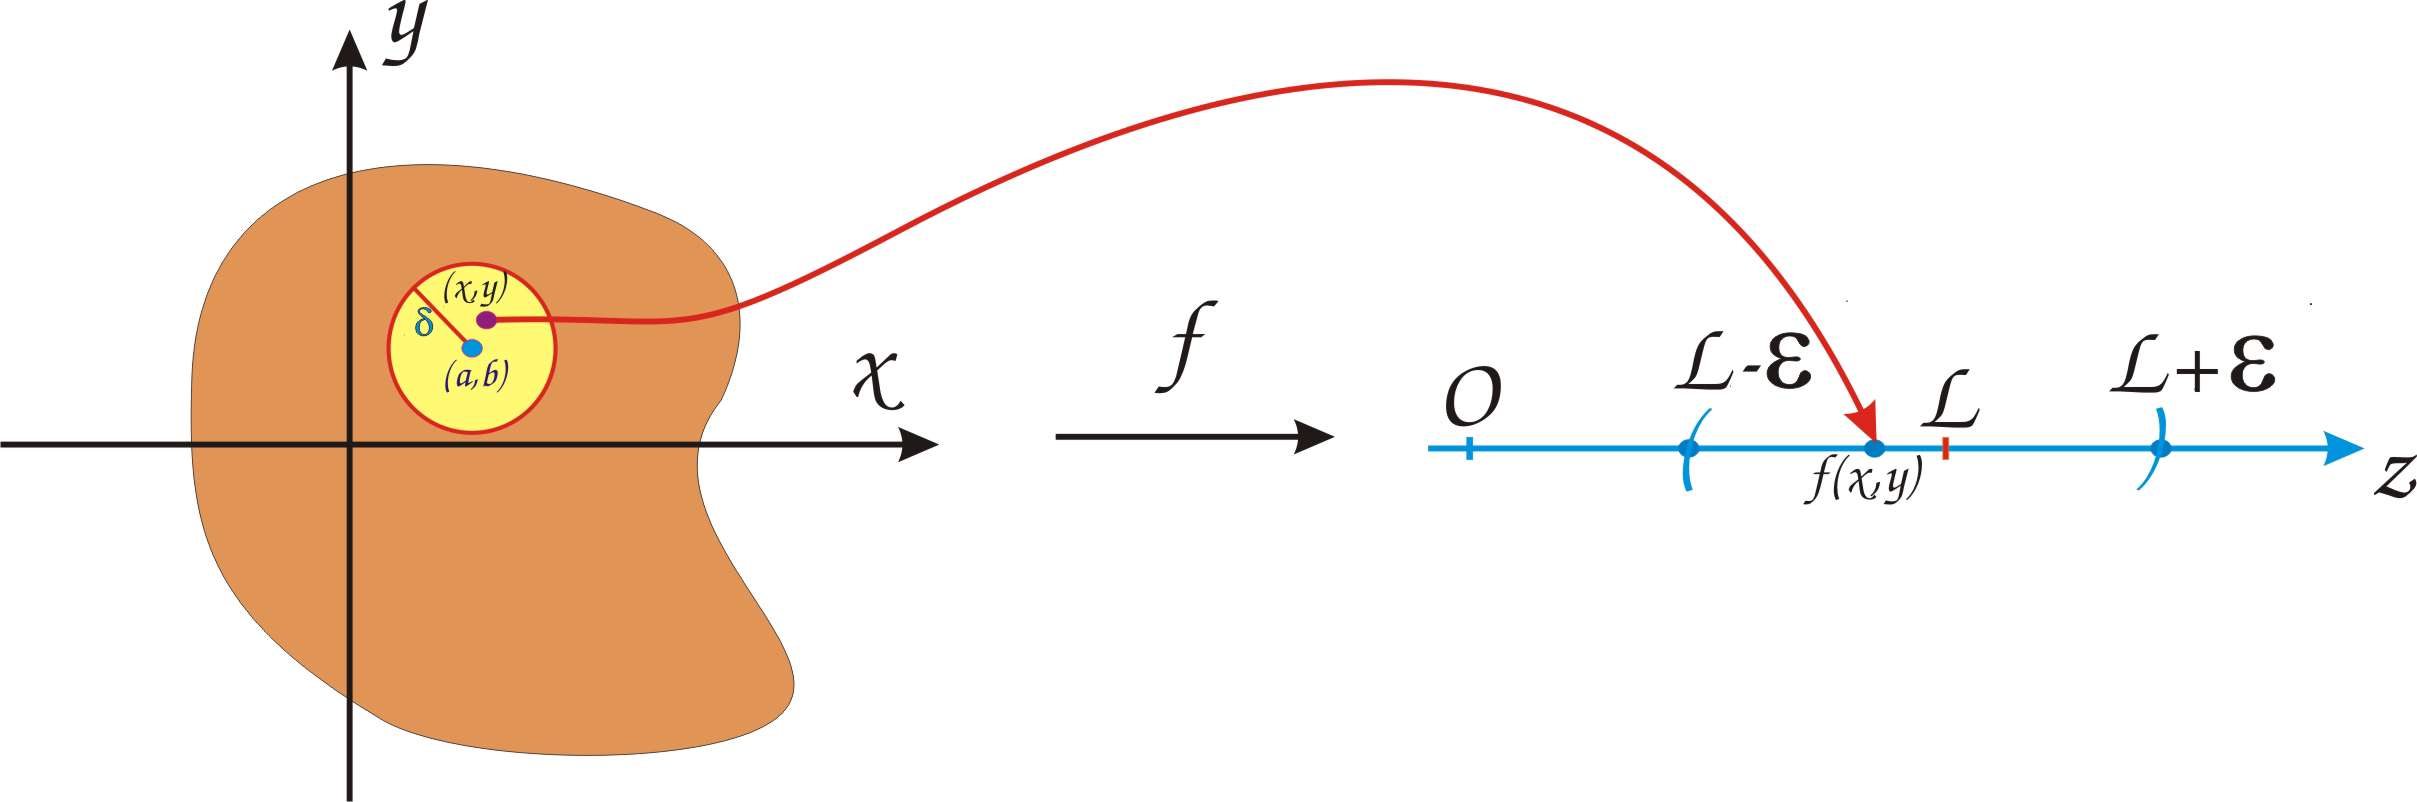
\includegraphics[scale = 0.28]{12.png}
    \captionof*{figure}{Ý nghĩa hình học của giới hạn hàm hai biến}
\end{center}
\DN \textbf{2.3.} Hàm hai biến $f$ được gọi là liên tục tại $(a,b)$ nếu như
\[
    \lim_{(x,y) \to (a,b)} f(x,y) = f(a,b).
\]
\DN \textbf{2.4.} Hàm hai biến $f$ gọi là liên tục trên miền $D$ nếu $f$ liên tục tại mọi điểm $(a,b) \in D$.
\subsection{Đạo hàm riêng.}
\subsubsection{Khái niệm.}
\[
\begin{gathered}
f: D \subset \mathbb{R}^2 \rightarrow \mathbb{R} \\
(x, y) \longmapsto f(x, y)
\end{gathered}
\]
Đạo hàm riêng cấp một của $f$ theo $x$ tại $(x_0,y_0)$:
\[
  f'_x(x_0,y_0) =  \frac{\partial f}{\partial x} (x_0,y_0) = \lim_{h \to 0} \dfrac{f(x_0 + h,y_0) - f(x_0,y_0)}{h}
\]
Đạo hàm riêng cấp một của $f$ theo $y$ tại $(x_0,y_0)$:
\[
    f'_y (x_0,y_0) = \frac{\partial f}{\partial y} (x_0,y_0) = \lim_{h \to 0} \dfrac{f(x_0y_0 + h) - f(x_0,y_0)}{h}
\]
%Cho hàm số $f: D \subset \mathbb{R}^2 \to \mathbb{R}$ xác định trên $D \subset \mathbb{R}^2$ và $(x_0,y_0) \in D$. Khi $x$ thay đổi, $y$ cố định $(y=y_0)$ thì ta được hàm một biến $x:g(x) = f(x,x_0)$. Nếu $g(x)$ có đạo hàm tại $x=x_0$ thì ta gọi đó là đạo hàm riêng của hàm $f(x,y)$ tại điểm $(x_0,y_0)$ theo biến $x$.\\
%\DN \textbf{2.5.} Số (nếu có) $\displaystyle\lim_{h \to 0} \dfrac{g(x_0 + h)-g(x_0)}{h}=\lim_{h \to 0} \dfrac{f(x_0 + h,y_0) - f(x_0,y_0)}{h}$ được gọi là đạo hàm riêng của hàm số $f(x,y)$ tại điểm $(x_0,y_0) \in G$ theo biến $x$. Đạo hàm riêng này được ký hiệu $f_{x}'(x_0,y_0)$ hoặc $\dfrac{\partial f}{\partial x}(x_0,y_0).$
%\begin{center}
%    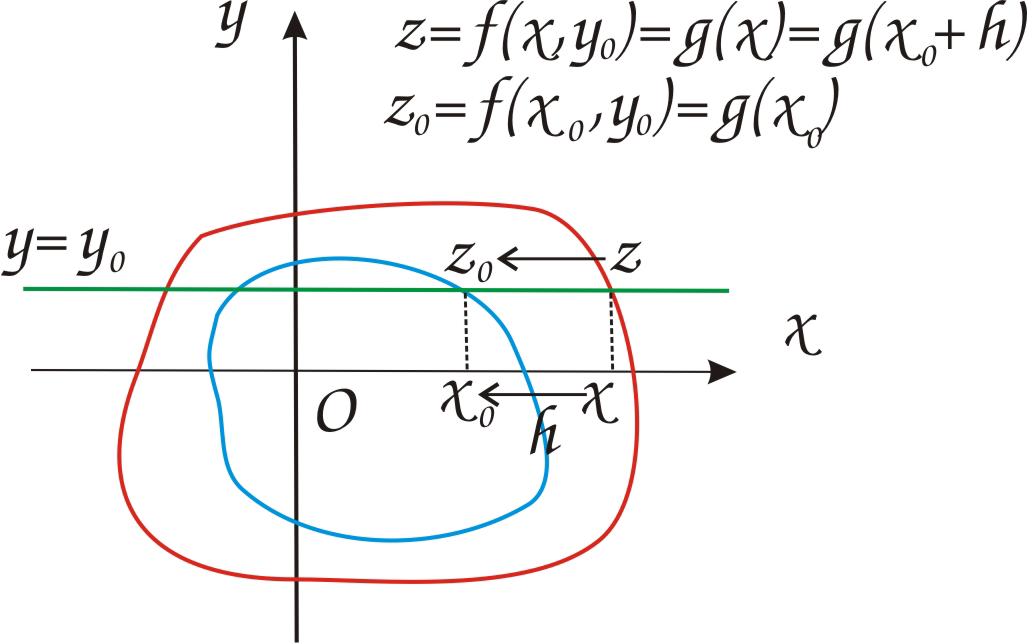
\includegraphics[scale = 0.3]{13.png}
%\end{center}
%\DN \textbf{2.6.} Số (nếu có) $\displaystyle\lim_{h \to 0} \dfrac{f(x_0,y_0 + h) - f(x_0,y_0)}{h}$ được gọi là đạo hàm riêng của hàm số $f(x,y)$ tại điểm $(x_0,y_0) \in G$ theo biến $y$. Đạo hàm riêng này được ký hiệu $f_{y}'(x_0,y_0)$ hoặc $\dfrac{\partial f}{\partial y}(x_0,y_0).$
\subsubsection{Quy tắc tìm đạo hàm riêng.}
\begin{enumerate}
    \item Để tìm $f_{x}'$ ta xem $y = const$ và lấy đạo hàm của $f(x,y)$ theo biến x.
    \item Để tìm $f_{y}'$ ta xem $x = const$ và lấy đạo hàm của $f(x,y)$ theo biến y.
\end{enumerate}
\subsubsection{Ý nghĩa hình học.}
Cho mặt cong $(S): z=f(x,y)$ và điểm $P(x_0,y_0,z_0)$ thuộc $(S)$.
\begin{itemize}
    \item $f'_x (x_0,y_0)$ là hệ số góc của tiếp tuyến $T_1$ với đường cong $(C_1)$ (giao tuyến của mặt cong $(S)$ với mặt phẳng $y=y_0$) tại $P$.
\end{itemize}
\begin{center}
    \includegraphics*[scale = 0.37]{T_1.png}
\end{center}
\begin{itemize}
    \item $f'_y (x_0,y_0)$ là hệ số góc của tiếp tuyến $T_2$ với đường cong $(C_2)$ (giao tuyến của mặt cong $(S)$ với mặt phẳng $x=x_0$) tại $P$.
\end{itemize}
\begin{center}
    \includegraphics*[scale = 0.38]{T_2.png}
\end{center}
\subsubsection{Ý nghĩa đạo hàm riêng.}
\begin{itemize}
    \item $f'_x$ là tốc độ thay đổi của $f$ theo hướng $Ox$ ($y$ không đổi).
    \item $f'_y$ là tốc độ thay đổi của $f$ theo hướng $Oy$ ($x$ không đổi).
\end{itemize}
Cho hàm số $f(x,y)$. Xét tại $(x_0,y_0)$
\begin{itemize}
    \item Khi $x_0 \gg 1, f'_x(x_0,y_0) \approx \Delta f$ khi $x$ tăng một đơn vị ($y$ không đổi).
    \item Khi $y_0 \gg 1, f'_y(x_0,y_0) \approx \Delta f$ khi $y$ tăng một đơn vị ($x$ không đổi).
\end{itemize}
\subsection{Mặt phẳng tiếp diện.}
\begin{center}
    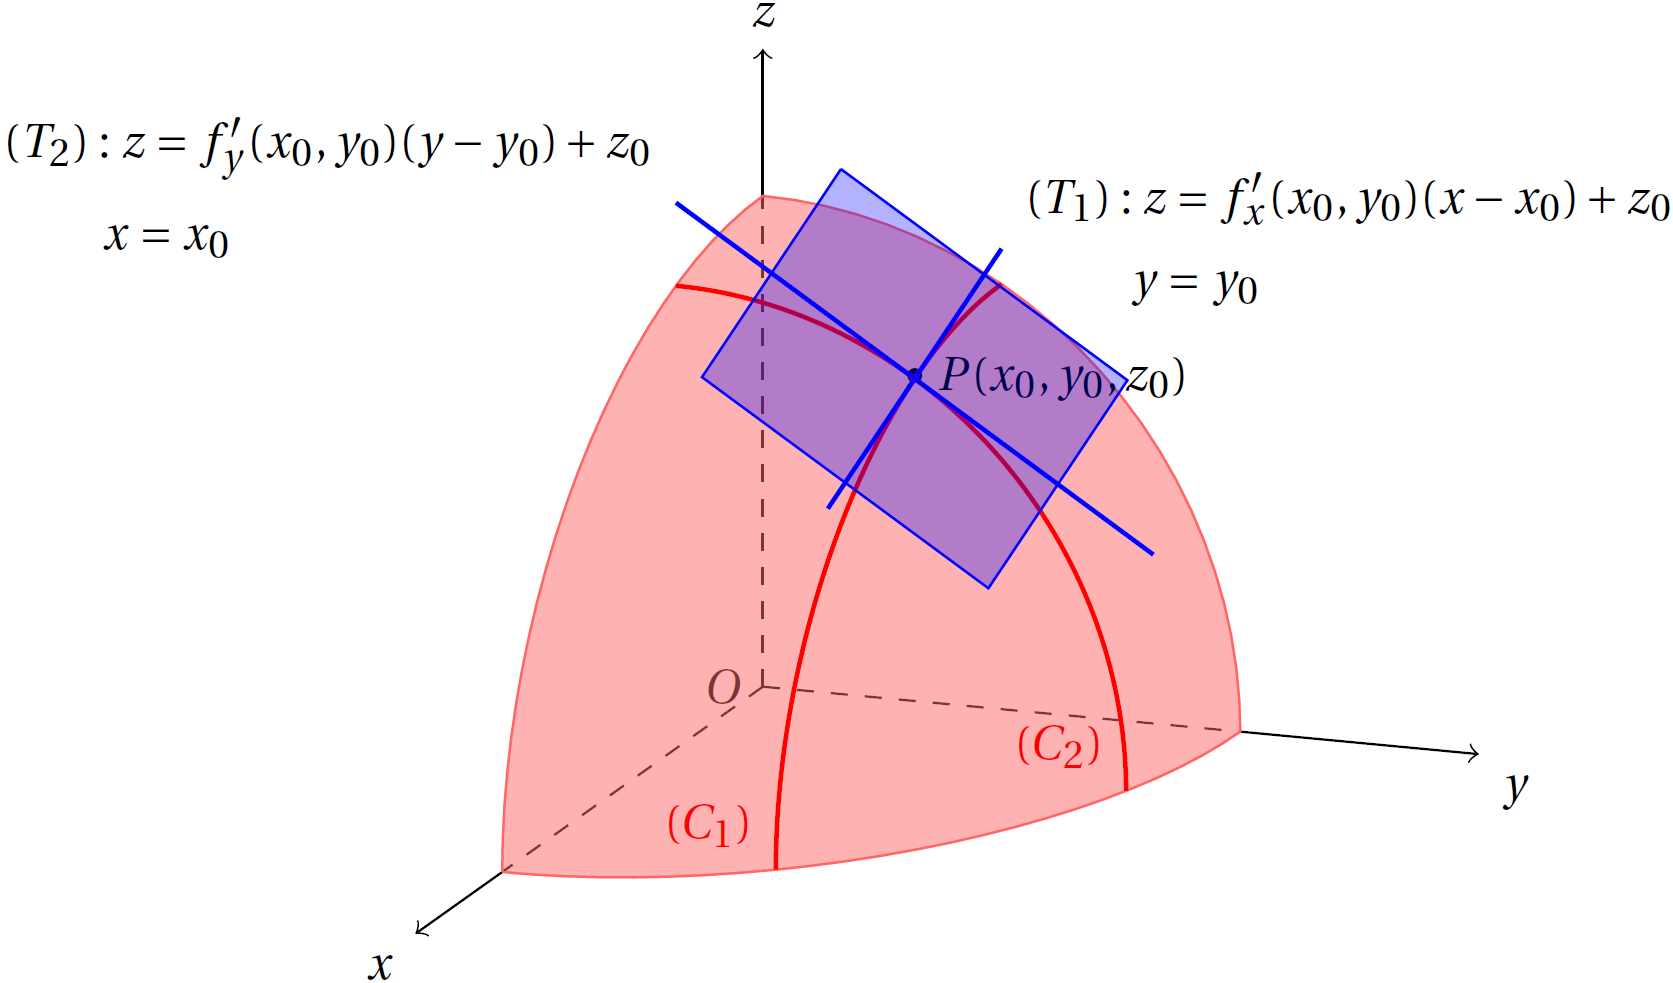
\includegraphics[scale = 0.38]{T_3.png}
    \captionof*{figure}{Mặt phẳng tiếp diện của mặt cong $z=f(x,y)$}
\end{center}
\DN \textbf{2.1.} Mặt phẳng tiếp diện với mặt cong $S$ tại điểm $P(x_0,y_0,z_0)$ là mặt phẳng chứa 2 tiếp tuyến $(T_1)$ và $(T_2)$.
\[
    f_{x}'(x_0,y_0)(x-x_0) + f_{y}'(x_0,y_0)(y-y_0) -(z-z_0)=0
\]
%\textit{\textbf{e.g.}} Tìm mặt phẳng tiếp diện với paraboloid elliptic $z=2x^2 + y^2$ tại $(1,1,3)$.
%\[
%    z-f(1,1)=f_{x}'(1,1)(x-1) + f_{y}'(1,1)(y-1) \Leftrightarrow z = 4x + 2y - 3    
%\]
\begin{itemize}
    \item vector chỉ phương của đường thẳng $T_2$: $\Vec{u}_2 = \left( 0;1;f'_y(x_0,y_0) \right)$
    \item vector chỉ phương của đường thẳng $T_1$: $\Vec{u}_1 = \left( 1;0;f'_x(x_0,y_0) \right)$
    \item Gọi $\Vec{n}$ là một vector pháp tuyến của tiếp diện $(S)$ tại $P$.
    \[
        \Vec{n} = \Vec{u}_2 \times \Vec{u}_1 = \left( f'_x(x_0,y_0);f'_y(x_0,y_0);-1 \right)
    \]
    \item Phương trình pháp tuyến của $S$ tại $P(x_0,y_0,z_0)$
    \[
        \frac{x-x_0}{f'_x(x_0,y_0)} = \frac{y-y_0}{f'_y(x_0,y_0)} = \frac{z-z_0}{-1}
    \]
\end{itemize}
\subsection{Đạo hàm riêng cấp cao.}
Cho hàm số $z =f(x,y)$. Đạo hàm riêng cấp 2 của $f$ là các đạo hàm riêng cấp một của $f_{x}'$ và $f_{y}'$.
\[
  \frac{\partial}{\partial x}\left( \frac{\partial f}{\partial x}\right) = \frac{\partial^2 f}{\partial x^2} = f_{xx}''; \quad \frac{\partial}{\partial y}\left( \frac{\partial f}{\partial x}\right) = \frac{\partial^2 f}{\partial x \partial y} = f_{xy}''
\]
\[
  \frac{\partial}{\partial x}\left( \frac{\partial f}{\partial y}\right) = \frac{\partial^2 f}{\partial y \partial x} = f_{yx}''; \quad \frac{\partial}{\partial y}\left( \frac{\partial f}{\partial y}\right) = \frac{\partial^2 f}{\partial y^2} = f_{yy}''    
\]
\textbf{Định lý 3.1.} \textit{Định lý Clairaut.} Cho hàm số $z =f(x,y)$ xác định trên miền $D$. Khi đó  nếu $f_{xy}''$ và $f_{yx}''$ là những hàm liên tục trên $D$ thì với mọi $(x_0,y_0) \in D$ ta có $f_{xy}'' (x_0,y_0) = f_{yx}'' (x_0,y_0)$.
%\subsubsection{Phương trình đạo hàm riêng.}
%\DN \textbf{2.7.} Phương trình đạo hàm riêng: 
%\[
%  \frac{\partial^2 u}{\partial x^2} + \frac{\partial^2 u}{\partial y^2} = 0
%\]
%được gọi là phương trình Laplace. Nghiệm của phương trình này được gọi là những hàm điều hòa, đóng vai trò trong những bài toán truyền nhiệt, lan truyền chất lỏng, điện trường,$\dots$

%\DN \textbf{2.8.} Phương trình đạo hàm riêng: 
%\[
%  \frac{\partial^2 u}{\partial t^2} =a^2 \frac{\partial^2 u}{\partial x^2}
%\]
%được gọi là phương trình sóng.
%-----------------------------------------------------------------
%\subsubsection{Sự xấp xỉ tuyến tính.}
%Trong ví dụ trên, mặt phẳng tiếp diện của hàm $f(x,y)=2x^2+y^2$ tại $(1,1,3)$ là $z=4x+2y-3$. Điều này có nghĩa là hàm tuyến tính $L(x,y)=4x+2y-3$ là sự xấp sỉ tốt nhất hàm $f(x,y)$ kh $(x,y)$ nằm gần $(1,1)$.
%\begin{center}  
%    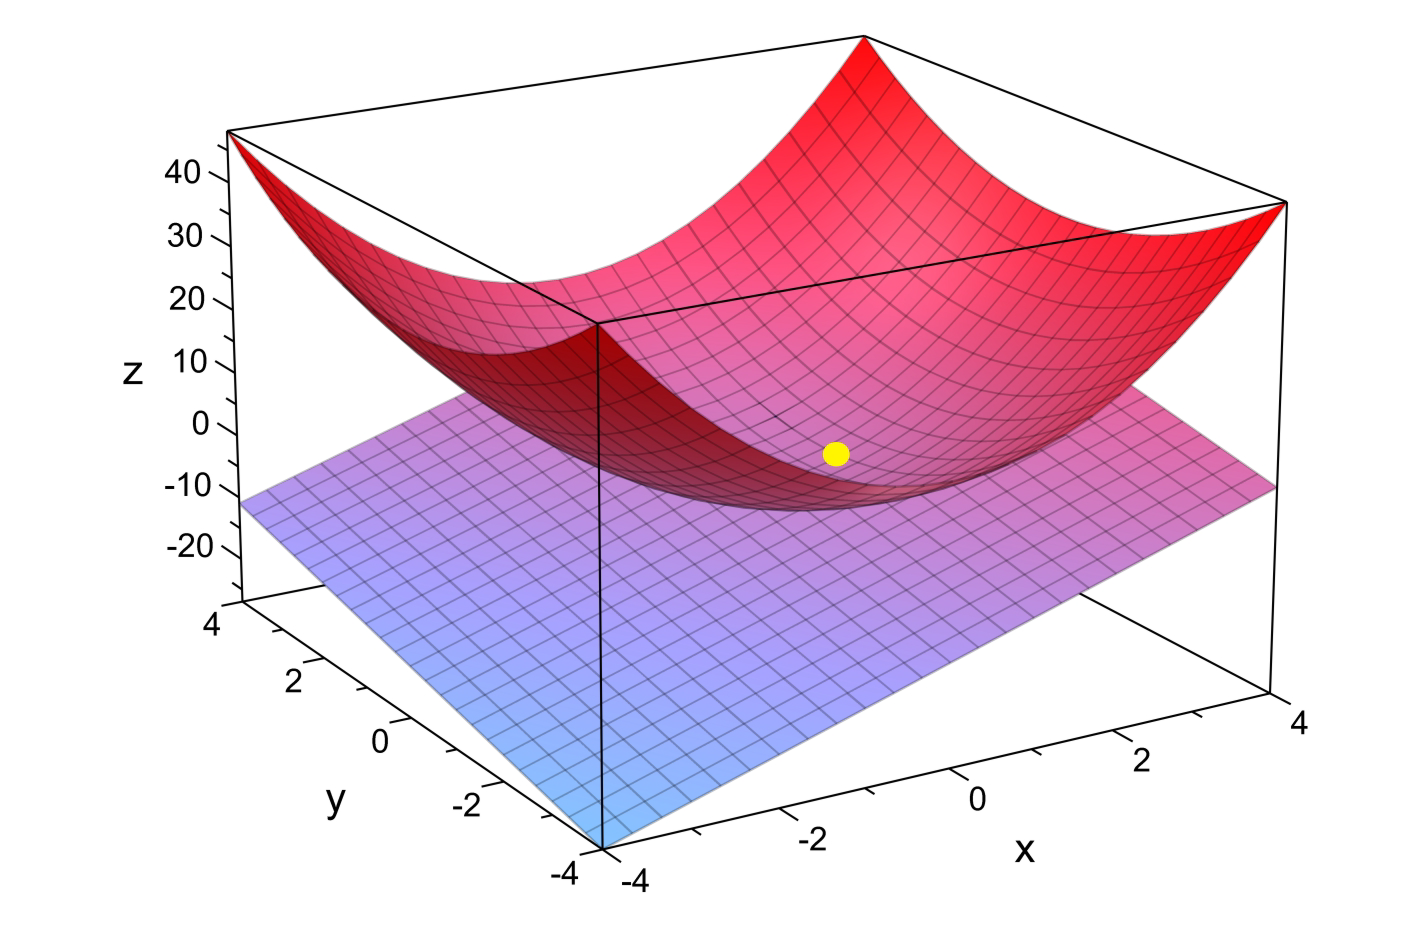
\includegraphics[scale = 0.28]{16.png}
%    \captionof*{figure}{Mặt Paraboloid $z=2x^2+y^2$ và mặt phẳng tiếp diện $z=4x+2y-3$ tại $(1,1,3)$}
%\end{center}
%Hàm tuyến tính $L(x,y)=4x+2y-3$ được gọi là hàm tuyến tính hóa của hàm $f$ tại điểm $(1,1)$ và sự xấp xỉ 
%\[
%    f(x,y) \approx 4x+2y-3    
%\]
%được gọi là sự xấp xỉ tuyến tính của hàm $f$ tại $(1,1)$.
%------------------------------------------------------------------------
\section{Sự khả vi và vi phân.}
Hàm số $f(x,y)$ được gọi là khả vi tại $(x_0,y_0)$ nếu 
\[
    f(x_0,\Delta x,y_0 + \Delta y) - f(x_0,y_0) = f'_x (x_0,y_0)\Delta x + f'_y (x_0,y_0)\Delta y + \alpha \Delta x + \beta \Delta y
\]
Điều kiện cần của khả vi: 
\begin{enumerate}
    \item $f$ khả vi tại $(x_0,y_0)$ thì $f$ liên tục tại $(x_0,y_0)$.
    \item $f$ khả vi tại $(x_0,y_0)$ thì $f$ có các đạo hàm riêng tại $(x_0,y_0)$ (tồn tại $f'_x, f'_y$).
\end{enumerate}

Cho hàm số $f(x,y)$. Công thức xấp xỉ tuyến tính của hàm số $f(x,y)$ tại $(x_0,y_0)$ là:
\[
    L(x,y) = f'_x(x_0,y_0)(x-x_0)+f'_y(x_0,y_0)(y-y_0)+f(x_0,y_0)
\]
\begin{center}
    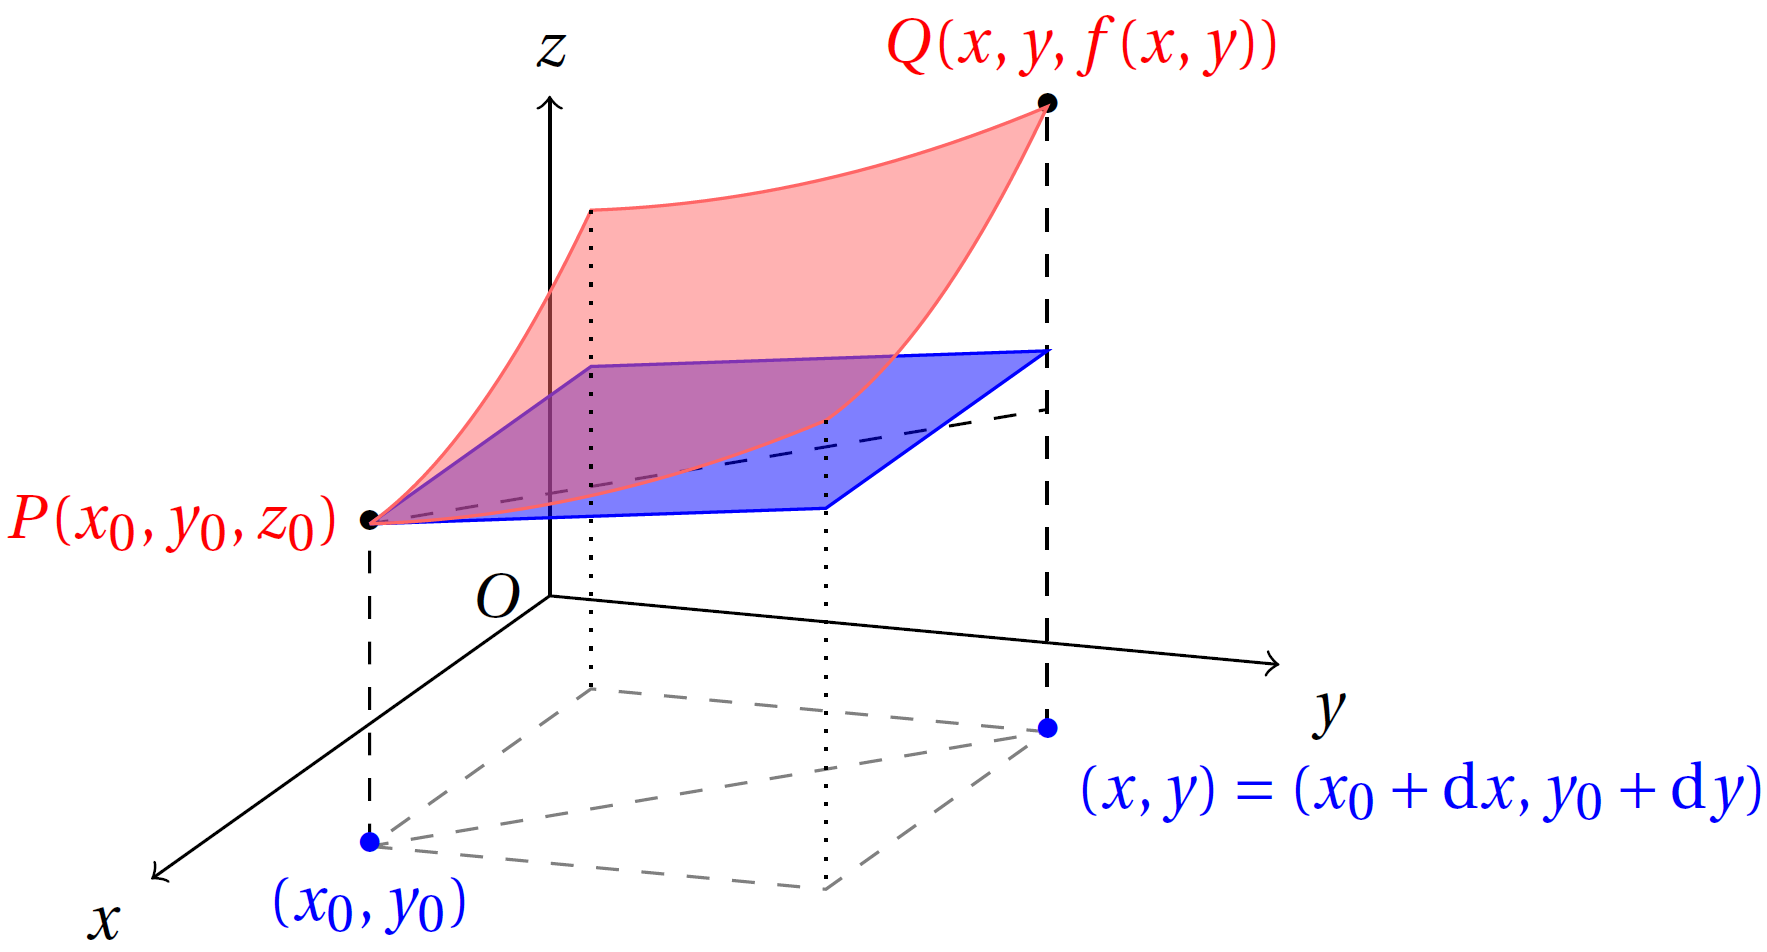
\includegraphics[scale = 0.38]{T_4.png}
\end{center}
Khi $(x,y)$ trong lân cận đủ nhỏ của $(x_0,y_0)$ thì $f(x,y) \approx L(x,y)$.
\subsubsection{Vi phân của hàm hai biến.}
\[
    df(x_0,y_0)=f'_x (x_0,y_0)dx + f'_y (x_0,y_0)dy    
\]

Đối với hàm số $f(x_1,x_2,\dots,x_n)$:
\[
    df = f'_{x_1} dx_1 + f'_{x_2} dx_2 + \cdots + f'_{x_n} dx_n    
\]
\subsubsection{Ý nghĩa vi phân.}
Cho mặt cong $(S):z=f(x,y)$ và điểm $P(x_0,y_0,z_0) \in (S)$.
\begin{center}
    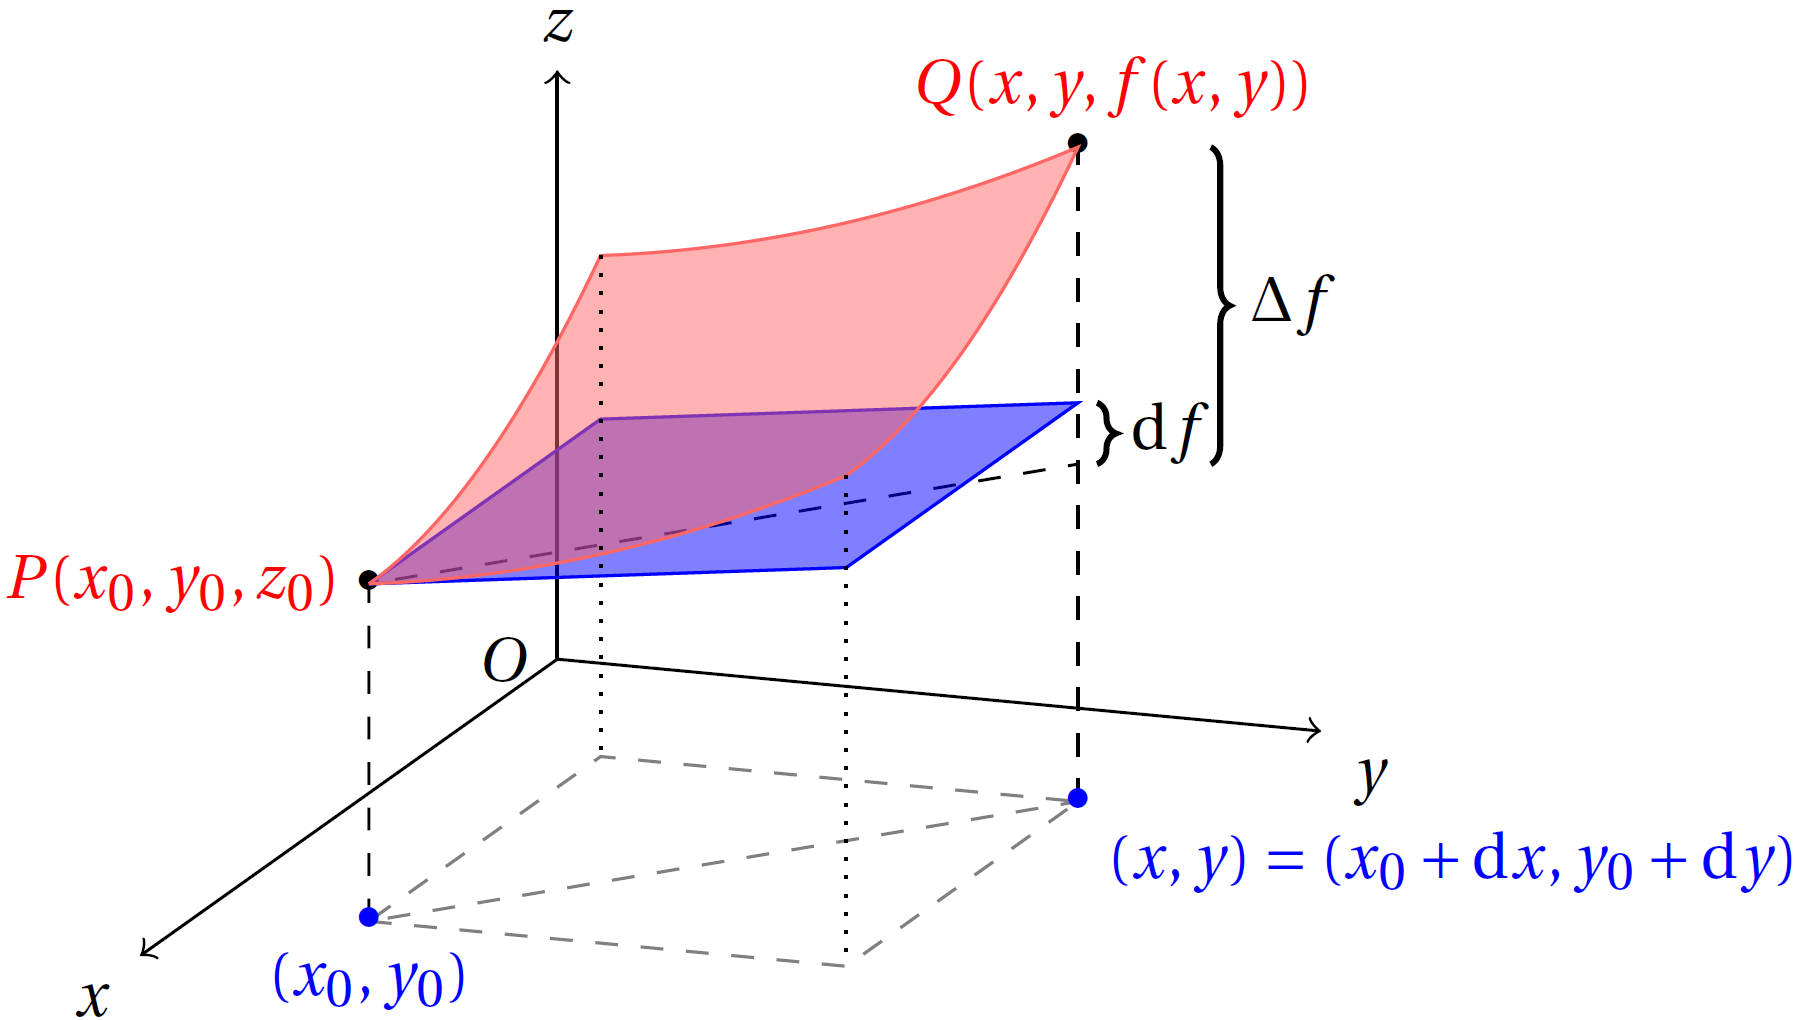
\includegraphics[scale = 0.38]{T_5.png}
\end{center}

Tiếp diện: $z=L(x,y)=f'_x(x_0,y_0)(x-x_0) + f'_y(x_0,y_0)(y-y_0) + z_0$.
\begin{itemize}
    \item $d f(x_0,y_0) = L(x,y) - z_0$.
    \item $\Delta f(x_0,y_0) = f(x,y) - z_0$.
\end{itemize}

Khi $(x,y)$ trong lân cận đủ nhỏ của $(x_0,y_0)$ thì $\Delta f \approx df$. %check slide 15 file Differential_DirectionalDerivative
%Ta có các công thức
%\[
%    d(f+g)=df+dg \qquad d(f.g)=g.df=f.dg \qquad d \left( \frac{f}{g} \right) =\frac{g.df-f.dg}{g^2}   
%\]
\subsubsection{Vi phân cấp cao.}
Vi phân cấp hai của $f$ là vi phân của $df(x,y)$ khi xem $dx,dy$ là $const$. $d^2 f(x,y)=d(df(x,y))$.
\[
    d^2 f(x,y) = f_{xx}''dx^2 + 2f_{xy}''dxdy + f_{yy}''dy^2
\]
Công thức tổng quát cho vi phân cấp cao.
\[
    d^n f(x,y) = \left( \frac{\partial}{\partial x}dx + \frac{\partial}{\partial y}dy \right)^n f(x,y)    
\]

\section{Đạo hàm theo hướng.}
Cho hàm số $z=f(x,y)$ vector đơn vị $u = \langle a,b \rangle$.
\begin{center}
    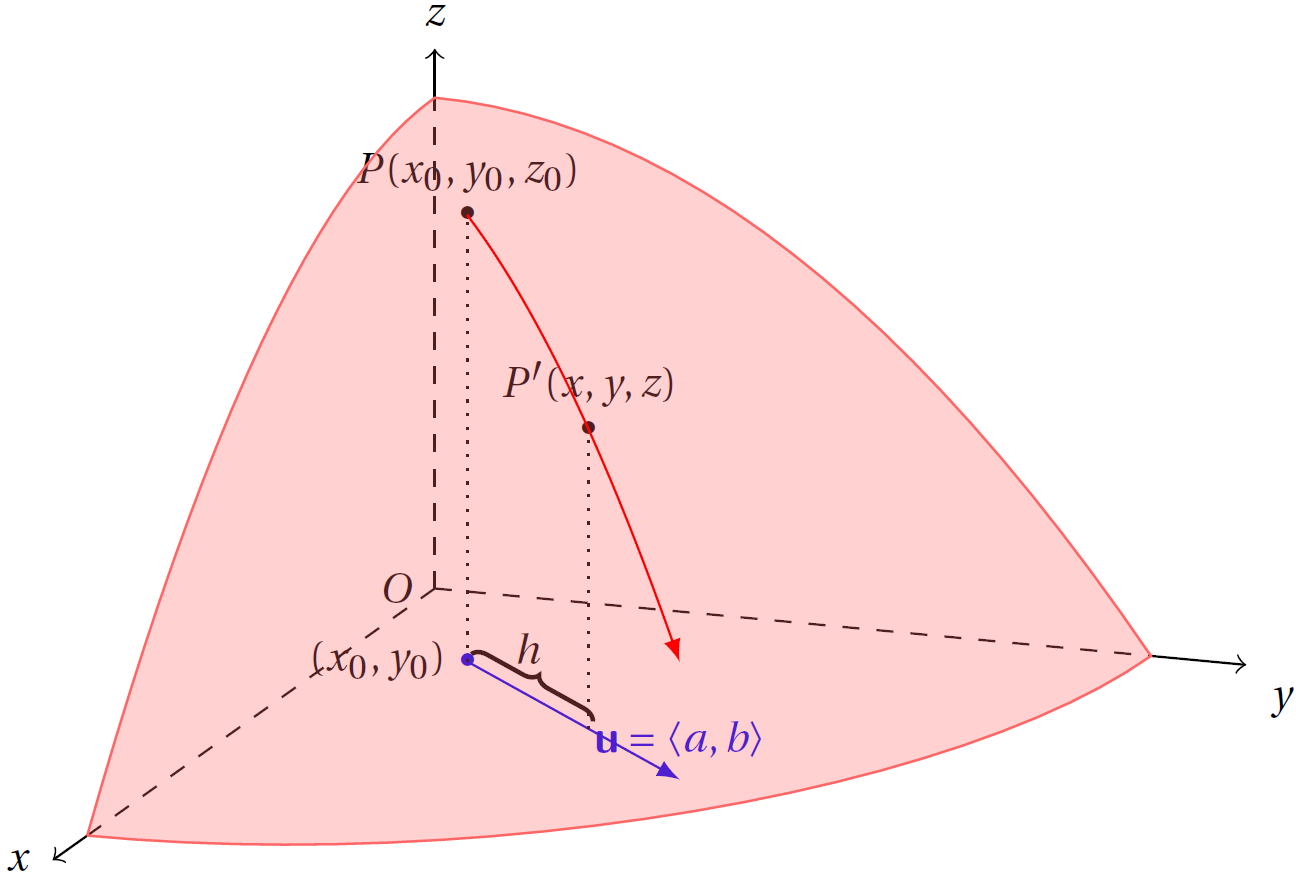
\includegraphics[scale = 0.38]{T_6.png}
\end{center}
Tốc độ thay đổi của $z$ theo hướng $u$:
\[
    \lim_{h \to 0}  \frac{\Delta z}{h} = \lim_{h \to 0} \frac{f((x_0,y_0) + h(a,b)) - f(x_0,y_0)}{h}
\]
Tốc độ thay dổi của $z$ khi $(x,y)$ thay đổi theo hướng $u$:
\[
    \lim_{h \to 0}  \frac{\Delta z}{h} = \lim_{h \to 0} \frac{f((x_0,y_0) + h(a,b)) - f(x_0,y_0)}{h}
\]
\[
    = \lim_{h \to 0} \frac{f(x_0 + ha, y_0 + hb) - f(x_0,y_0)}{h}    
\]
Giới hạn này (nếu tồn tại) được gọi là đạo hàm của $f$ theo hướng vector $u$ tại $(x_0,y_0)$.

\textul{Note:} $u = \langle u_1,u_2,\dots,u_n \rangle$ là một vector đơn vị thỏa $(u_1)^2+(u_2)^2+\ldots +(u_n)^2 = 1$.\\
Cho hàm số $f(x,y)$. Với $u = \langle a,b \rangle$ là một vector đơn vị. Đạo hàm của $f$ theo hướng $u$ tại $(x_0,y_0)$:
\[
    f'_u(x_0,y_0) = \lim_{h \to 0} \frac{f(x_0 + ha, y_0 + hb) - f(x_0,y_0)}{h}
\]
Nếu $f$ khả vi tại $(x_0,y_0)$ thì:
\[
     f'_{u} (x,y) = f'_x (x,y).a + f'_y (x,y).b      
\]
Ý nghĩa hình học: Đạo hàm theo hướng là hệ số góc của tiếp tuyến đối với đường cong tại 1 điểm.
\section{Mối liên hệ giữa vector Gradient và đạo hàm theo hướng.}
\subsection{Vector Gradient.}
Cho $z=f(x,y)$, khi đó véc-tơ gradient của hàm số $f$ được xác định như sau:
\[
    \bigtriangledown f(x,y) = \langle f'_x (x,y),f'_y (x,y) \rangle
\]
\subsection{Vector Gradient - Đạo hàm theo hướng.}
Cho $f$ khả vi tại $(x_0,y_0)$, vector đơn vị $u = \langle a,b \rangle$.
\[
    f'_u(x_0,y_0) = f'_x(x_0,y_0).a + f'_y(x_0,y_0).b    
\]
\[
    \bigtriangledown f(x_0,y_0) = \left( f'_x(x_0,y_0),f'_y(x_0,y_0) \right)    
\]
\begin{center}
    \fbox{$f'_u = \bigtriangledown f \cdot u = |\bigtriangledown f| \cdot |u| \cdot \cos(\bigtriangledown f,u) = |\bigtriangledown f| \cdot \cos(\bigtriangledown f,u) $}    
\end{center}
Cho $f$ là hàm khả vi 2 hoặc 3 biến. GTLN của đạo hàm theo hướng $\Vec{u}$: $f'_{\Vec{u}}$ là $|\bigtriangledown f|$ đạt được khi $\Vec{u} \uparrow \uparrow \bigtriangledown f$. GTNN của đạo hàm theo hướng $\Vec{u}$: $f'_{\Vec{u}}$ là $-|\bigtriangledown f|$ đạt được khi $\Vec{u}$ ngược hướng $\bigtriangledown f$.
\section{Đạo hàm riêng và vi phân của hàm hợp.}
$\bullet$ Cho $z = f(x,y)$ và $x=x(u,v), y=y(u,v) \Rightarrow z = z(u,v)$. Nếu $z,x,y$ khả vi:
\begin{center}
    \fbox{$z_u '= f'_x.x'_u + f'_y.y'_u \qquad z_v '= f'_x.x'_v + f'_y.y'_v $}
\end{center}
Tổng quát hơn ta có 2 công thức sau:
\begin{center}
    \fbox{$\dfrac{\partial z}{\partial u} = \dfrac{\partial f}{\partial x}\dfrac{\partial x}{\partial u} + \dfrac{\partial f}{\partial y}\dfrac{\partial y}{\partial u} \qquad \dfrac{\partial z}{\partial v} = \dfrac{\partial f}{\partial x}\dfrac{\partial x}{\partial v} + \dfrac{\partial f}{\partial y}\dfrac{\partial y}{\partial v}$}
\end{center}
Vi phân của hàm hợp: 
\[
    \begin{aligned}
        &dz = z'_u du + z'_v dv \\
        &dz = (f'_x.x'_u + f'_y.y'_u)du + (f'_x.x'_v + f'_y.y'_v)dv\\
        &dz = f'_x(x'_u du + x'_v dv) + f'_y(y'_u du + y'_v dv)   
    \end{aligned}    
\]

$\bullet$ \textbf{Trường hợp riêng 1.} Cho $z = f(x),\thickspace x = x(u,v) \Rightarrow z=z(u,v)$ (hợp của 1 biến và 2 biến).
\begin{center}
    \fbox{$ z'_u = f'(x).x'_u \qquad z'_v = f'(x).x'_v$}
\end{center}
\[
    \begin{aligned}
        &dz = z'_u du + z'_v dv \\
        \Longrightarrow &dz = f'(x)dx = f'(x)(x'_u du + x'v dv)
    \end{aligned}    
\]

$\bullet$ \textbf{Trường hợp riêng 2.} $z = f(x,y),\thickspace x = x(t),\thickspace y = y(t) \Rightarrow z = z(t)$ (hợp 2 biến và 1 biến).
\begin{center}
    \fbox{$z'(t) = f'_x.x'(t) + f'_y.y'(t)$}
\end{center}
\[
    \begin{aligned}
        &dz = z'(t) dt \\
        &dz = f'_x dx + f'_y dy = f'_x.x'(t) dt + f'_y.y'(t) dt
    \end{aligned}
\]

$\bullet$ \textbf{Trường hợp riêng 3.} $z=f(x,y),\thickspace y= y(x) \Rightarrow z = z(x)$ (hợp 2 biến và 1 biến).
\begin{center}
    \fbox{$ z'(x) = f'_x + f'_y.y'(x)$}
\end{center}
\[
    dz = z'(x) dx    
\]
\textcolor{red}{\textbf{Lưu ý:}} Khi tính đạo hàm hàm hợp, luôn bắt đầu từ  đạo hàm của $f$ theo biến chính. Sau đó, tùy thuộc vào yêu cầu, nhân thêm đạo hàm của biến chính vào cạnh đạo hàm của $f$.
\subsection{Đạo hàm và vi phân hàm ẩn.}
Hàm số $y=y(x)$ được cho bởi phương trình $F(x,y) = 0$. Đạo hàm của hàm ẩn 1 biến $y=y(x)$:
\[
    y'(x) = -\frac{F'_x}{F'_y}    
\]

Liên hệ tìm pháp vector của đường cong: Cho đường cong $y=y(x)$ xác định bởi phương trình $F(x,y)=0$. Phương trình tiếp tuyến tại $(x_0,y_0)$:
\[
    y-y_0 = y'(x_0)(x-x_0)    
\]
\[
    F'_x(x_0,y_0)(x-x_0) + F'_y(x_0,y_0)(y-y_0) = 0
\]
\[
    \Vec{n} = \bigtriangledown F(x_0,y_0) = ( F'_x(x_0,y_0), F'_y(x_0,y_0) )   
\]

Hàm số $z=z(x,y)$ xác định từ phương trình $F(x,y,z) = 0$ ($x,y,z$ là các biến độc lập khi tính $F'_x,F'_y,F'_z$). Đạo hàm của hàm ẩn 2 biến $z=z(x,y)$
\[
    z'_x = -\frac{F'_x}{F'_z} \qquad z'_y = -\frac{F'_y}{F'_z}
\]

Liên hệ tìm pháp vector của mặt cong: Cho mặt cong $z=z(x,y)$ xác định bởi phương trình $F(x,y,z) = 0$. Phương trình tiếp diện tại $(x_0,y_0,z_0)$
\[
    z'_x(x_0,y_0)(x-x_0) + z'_y(x_0,y_0)(y-y_0) + (z-z_0)= 0
\]
\[
    F'_x(x_0,y_0,z_0)(x-x_0) + F'_y(x_0,y_0,z_0)(y-y_0) + F'_z(x_0,y_0,z_0)(z-z_0) = 0   
\]
\[
    \Vec{n} = \bigtriangledown F(x_0,y_0,z_0) = ( F'_x(x_0,y_0,z_0), F'_y(x_0,y_0,z_0), F'_z(x_0,y_0,z_0) )   
\]
\subsection{Công thức Taylor và Maclaurin.}
\section{Cực trị hàm nhiều biến.}
\subsection{Cực trị tự do.}
\[
\begin{gathered}
f: D \subset \mathbb{R}^2 \rightarrow \mathbb{R} \\
(x, y) \longmapsto f(x, y)
\end{gathered}
\]
$f$ đạt cực đại tại $P(x_0,y_0)$ nếu tồn tại một lân cận $B(P,r)$ của $P(x_0,y_0)$ sao cho
\[
    f(x.y) \leq f(x_0,y_0), \qquad \forall (x,y) \in B(P,r)    
\]
$f$ đạt cực đại chặt tại $P(x_0,y_0)$ nếu tồn tại một lân cận $B(P,r)$ của $P(x_0,y_0)$ sao cho
\[
    f(x.y) < f(x_0,y_0), \qquad \forall (x,y) \in B(P,r) \backslash \lbrace (x_0,y_0) \rbrace   
\]
$f$ đạt cực tiểu tại $P(x_0,y_0)$ nếu tồn tại một lân cận $B(P,r)$ của $P(x_0,y_0)$ sao cho
\[
    f(x.y) \geq f(x_0,y_0), \qquad \forall (x,y) \in B(P,r)    
\]
$f$ đạt cực trị tại $P(x_0,y_0)$ nếu $f$ đạt cực đại hoặc cực tiểu tại $P(x_0,y_0)$
\begin{comment}
    \pgfplotsset{width=10cm,compat=1.18}
\begin{tikzpicture}
        \begin{axis}[colormap/Blues ,title= \text{$z = -xye^{-x^2-y^2}$}]
        \addplot3[surf, samples = 50]{-x*y*exp(-x^2-y^2)};
        \end{axis}
\end{tikzpicture}
\textbf{Định lý.} (Điều kiện cần) Nếu hàm số $f(x,y)$ có cực trị tại $(x_0,y_0)$ và các đạo hàm riêng cấp một của $f$ tại $(x_0,y_0)$ tồn tại thì 
\[
    f'_x(x_0,y_0) = 0 \text{ và } f'_y (x_0,y_0) = 0    
\]
Cho hàm số $f(x,y)$. Nếu $f'_x(x_0,y_0) = 0$ và $f'_y(x_0,y_0) = 0$ thì $(x_0,y_0)$ được gọi là điểm dừng.

\textbf{Định lý.} (Điều kiện đủ) Cho hàm số $f(x,y)$ có đạo hàm riêng liên tục đến cấp 2 trong một lân cận của điểm dừng $P(x_0,y_0)$
\[
    d^2 f(P) = f''_{xx} (P) dx^2 + 2f''_{xy} (P)dxdy + f''_{yy} (P) dy^2 
\]
\begin{itemize}
    \item Nếu $d^2 f(P)$ là dạng toàn phương xác định dương thì $P(x_0,y_0)$ là điểm cực tiểu.
    \item Nếu $d^2 f(P)$ là dạng toàn phương xác định âm thì $P(x_0,y_0)$ là điểm cực đại.
\end{itemize}
\textbf{Các bước tìm cực trị:}
\begin{enumerate}
    \item Cho $f(x,y)$. Tìm $f'_x (x,y)=0$, $f'_y (x,y)=0 \Rightarrow $ điểm dừng $(x_0,y_0)$.
    \item Tính $\Delta = f''_{xx}.f''_{yy} - \left( f''_{xy} \right)^2$.
    \begin{itemize}
        \item TH1: $\Delta > 0$. Nếu $f''_{xx} > 0 \Rightarrow$ cực tiểu, $f''_{xx} < 0 \Rightarrow$ cực đại.
        \item TH2: $\Delta = 0 \Rightarrow$ Xét dấu $f(x,y) - f(x_0,y_0)$.
        \item TH3: $\Delta < 0 \Rightarrow$ Điểm yên ngựa.
    \end{itemize}
\end{enumerate}
\subsection{Cực trị có điều kiện.}
$f$ đại cực đại có điều kiện tại $P(x_0,y_0)$ với điều kiện $\varphi (x,y) = 0$ nếu tồn tại một lân cận $B(P,r)$ của $(x_0,y_0)$ sao cho:
\[
    f(x,y) \leq f(x_0,y_0), \qquad \forall (x,y) \in B(P,r) \text{ và } \varphi (x,y) = 0    
\]
\textbf{Các bước tìm cực trị có điều kiện.} Dùng phương pháp nhân tử Larange $L(x,y) = f(x,y) + \lambda.\varphi (x,y)$
\begin{enumerate}
    \item Tìm điểm dừng $L(x,y)$: $L'_x (M_0) = 0, L'_y (M_0) = 0, \varphi (M_0) = 0$.
    \item Xét dấu $d^2 L$ tại $M_0$ kèm điều kiện $d \varphi (M_0) = 0$.
    \begin{itemize}
        \item Xác định dương: cực tiểu.
        \item Xác định âm: cực đại.
    \end{itemize}
\end{enumerate}
\subsection{Giá trị lớn nhất - Giá trị nhỏ nhất.}
Cho D là một tập khác rỗng trong $\mathrm{R}^n$.

$X$ là một điểm dính của D nếu mọi quả cầu tâm $X$ đều chứa ít nhất một phần tử của D.

D là một tập đóng trong $\mathrm{R}^n$ nếu mọi điểm dính của D đều thuộc D.
\begin{center}
    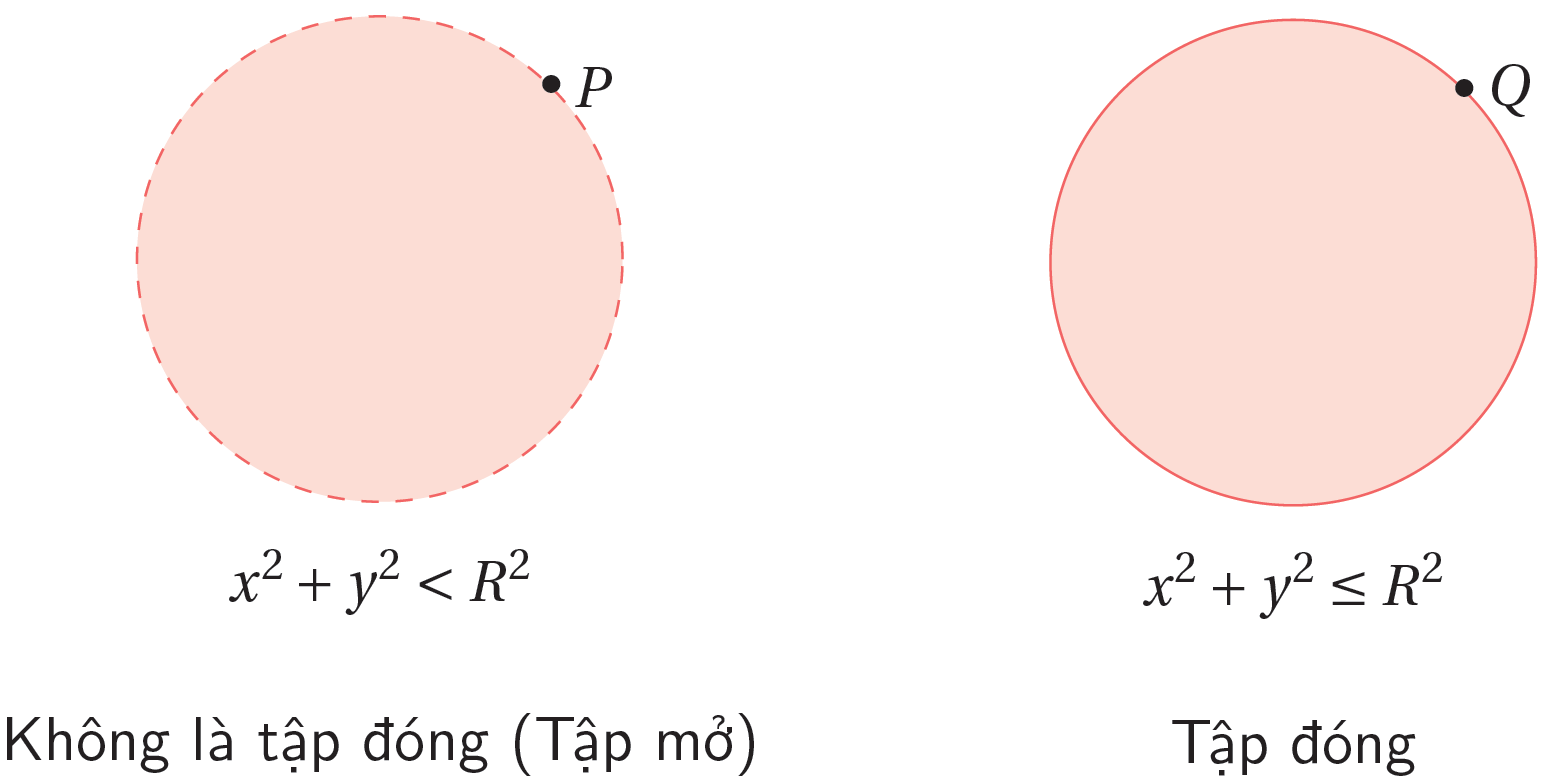
\includegraphics[scale = 0.38]{T_7.png}
\end{center}
D là một tập bị chặn nếu D nằm trong một quả cầu trong $\mathrm{R}^n$.
\begin{center}
    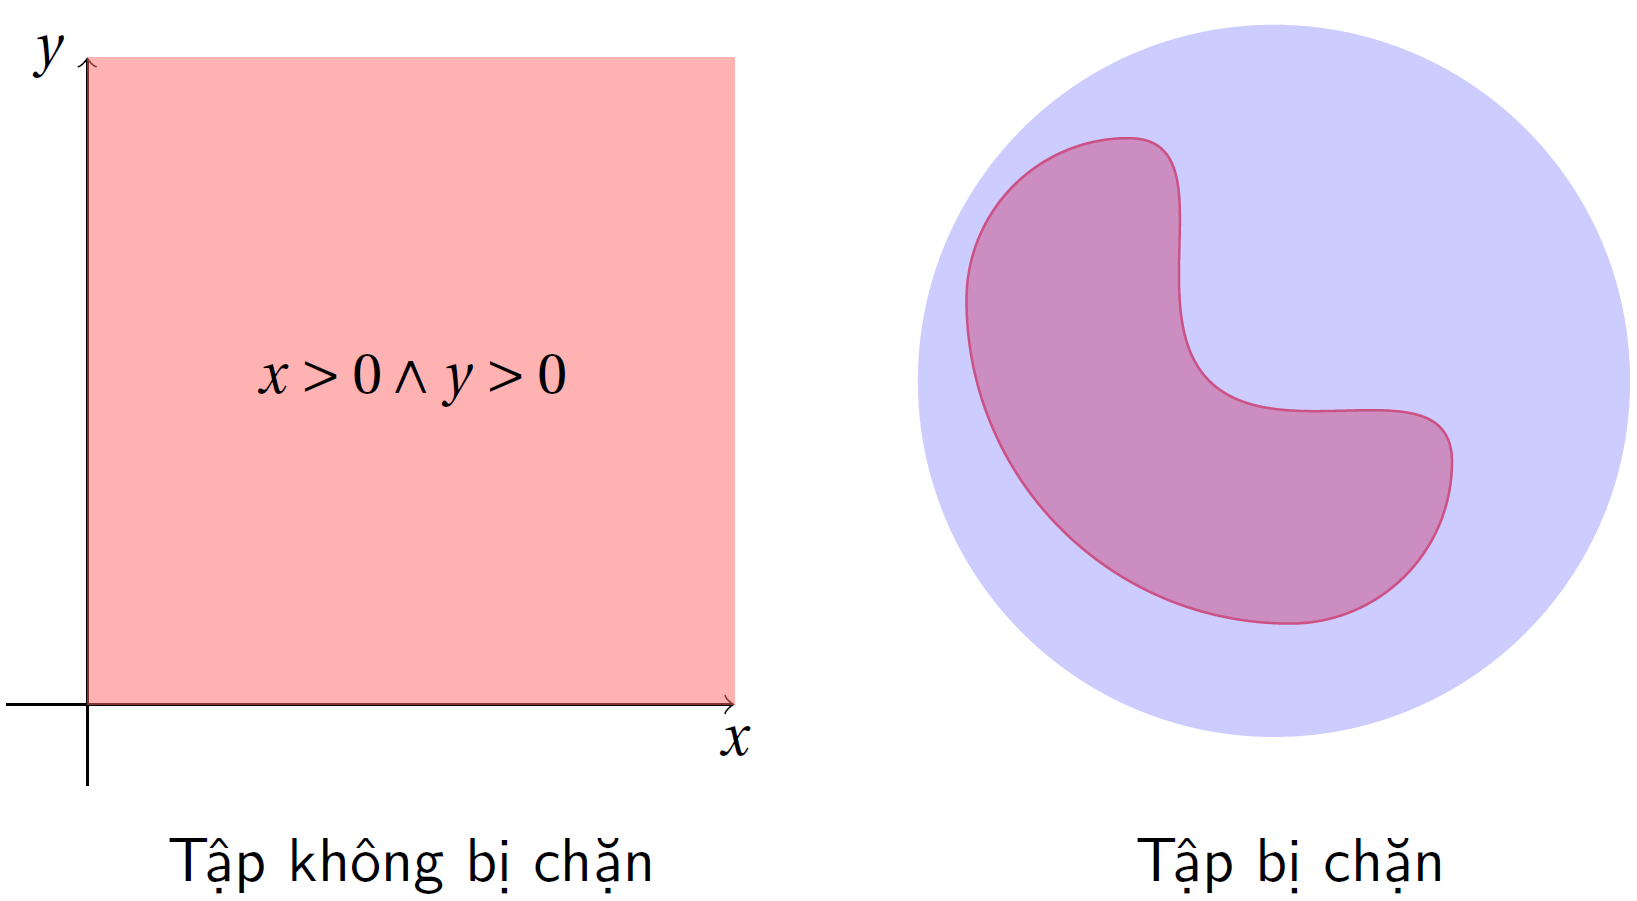
\includegraphics[scale = 0.38]{T_8.png}
\end{center}
D là một tập compact trong $\mathrm{R}^n$ nếu D là tập đóng và bị chặn trong $\mathrm{R}^n$.

\textbf{Định lý.} Nếu hàm số $f$ liên tục trên tập compact D thì $f$ luôn có giá trị lớn nhất (GTLN) và giá trị nhỏ nhất (GTNN) trên D. 

\textbf{\textul{Phương pháp tìm GTLN - GTNN của $f$ trên tập compact $D \subset \mathrm{R}^2$}}
\begin{itemize}
    \item Bước 1: Tìm điểm tới hạn của $f$ trên miền trong của D (D bỏ đi biên).
    \item Bước 2: Tìm điểm tới hạn cảu $f$ trên biên $\varphi(x,y) = 0$ (Tìm điểm dừng và điểm mà tại đó các đạo hàm riêng không xác định với điều kiện $\varphi (x,y) = 0$).
    \item Bước 3: So sánh giá trị của $f$ tại các điểm trên.
\end{itemize}
\newpage
\chapter{TÍCH PHÂN KÉP}
\section{Định nghĩa.}
Cho hàm số $f(x,y) \geq 0, \forall (x,y) \in D$. Tích phân kép của hàm số $f(x,y)$ trên miền $D$ là: 
\[
    \iint_{D} f(x,y) dxdy  = \iint_D f(x,y) dA = \lim_{m,n \to \infty} \sum_{i=1}^{m} \sum_{j=1}^{n} f(x_i^*, y_i^*) \Delta x \Delta y
\]
nếu giới hạn này tồn tại. Lúc này $f(x,y)$ được gọi là hàm khả tích trên $D$.

\textbf{Tính chất.}
\[
    S(D) = \iint_D dxdy    
\]
\[
    \iint_D \alpha.f(x,y)dxdy = \alpha \iint_D f(x,y)dxdy    
\]
\[
    \iint_D (f+g) dxdy = \iint_D fdxdy  + \iint_D gdxdy
\]
\end{comment}

\end{document}